\documentclass[12pt,a4paper]{report}

\usepackage{microtype}
\tolerance=1000
\emergencystretch=2em
\hbadness=5000
\hyphenpenalty=10000
\exhyphenpenalty=10000

\usepackage{array}
\usepackage{tabularx}
\usepackage{float}
\usepackage{graphicx}
\graphicspath{{figures/}{./}}
\usepackage{amsmath}
\usepackage{amssymb}
\usepackage{subcaption}
\usepackage{booktabs}
\usepackage{xcolor}

%--------------------------------
% Page Margins
%--------------------------------
\usepackage[
a4paper,
left=1in,
right=1in,
top=1in,
bottom=1in,
includehead,
includefoot,
headheight=16pt
]{geometry}

%--------------------------------
% Font (pdfLaTeX Compatible)
%--------------------------------
\usepackage[T1]{fontenc}
\usepackage[utf8]{inputenc}
\usepackage{mathptmx}

%--------------------------------
% Line Spacing
%--------------------------------
\usepackage{setspace}

%--------------------------------
% Paragraph Formatting
%--------------------------------
\setlength{\parindent}{0pt}
\setlength{\parskip}{2pt plus 1pt minus 1pt}

%--------------------------------
% Headings
%--------------------------------
\usepackage{titlesec}

% List gap - globally tighten itemize and enumerate lists
\usepackage{enumitem}
\setlist{itemsep=1.5pt, parsep=0pt, topsep=3pt, partopsep=0pt}
\setlist[itemize]{itemsep=1.5pt, parsep=0pt, topsep=3pt, partopsep=0pt}
\setlist[enumerate]{itemsep=1.5pt, parsep=0pt, topsep=3pt, partopsep=0pt}
%--------------------------------
% Header & Footer
%--------------------------------
\usepackage{fancyhdr}

\pagestyle{fancy}
\fancyhf{}

\fancyhead[R]{Real-Time Network Intrusion Detection and Alert System}

\fancyfoot[L]{Department of Computer Applications, MACE}
\fancyfoot[R]{\thepage}

\renewcommand{\headrulewidth}{0.4pt}
\renewcommand{\footrulewidth}{0.4pt}

\fancypagestyle{plain}{
    \fancyhf{}
    \fancyhead[R]{Real-Time Network Intrusion Detection and Alert System}
    \fancyfoot[L]{Department of Computer Applications, MACE}
    \fancyfoot[R]{\thepage}
    \renewcommand{\headrulewidth}{0.4pt}
    \renewcommand{\footrulewidth}{0.4pt}
}

%--------------------------------
% Float & Table Spacing
%--------------------------------
\setlength{\intextsep}{6pt}        % Tightens space above and below [H] tables
\setlength{\textfloatsep}{8pt}     % Space between floating tables and text
\setlength{\floatsep}{6pt}         % Space between consecutive tables
\setlength{\abovecaptionskip}{8pt} % Space above caption
\setlength{\belowcaptionskip}{0pt} % Space below caption

%--------------------------------
% Chapter Formatting
%--------------------------------
\titleformat{\chapter}
{\normalfont\bfseries\fontsize{16}{20}\selectfont}
{\thechapter.}{1em}{}

\titleformat{name=\chapter,numberless}
{\normalfont\bfseries\fontsize{16}{20}\selectfont\filcenter}
{}{0pt}{}

\titlespacing*{\chapter}
{0pt}
{-30pt}
{2pt}

\titlespacing*{name=\chapter,numberless}
{0pt}
{-30pt}
{15pt}

%--------------------------------
% Section Formatting
%--------------------------------
\titleformat{\section}
{\normalfont\bfseries\fontsize{14}{18}\selectfont}
{\thesection}{1em}{}

\titlespacing*{\section}
{0pt}
{2pt}
{2pt}

%--------------------------------
% Subsection Formatting
%--------------------------------
\titleformat{\subsection}
{\normalfont\bfseries\fontsize{12}{16}\selectfont}
{\thesubsection}{1em}{}

\titlespacing*{\subsection}
{0pt}
{2pt}
{2pt}

%--------------------------------
% Begin Document
%--------------------------------
\begin{document}
\onehalfspacing

%==================================================================================================================
% FRONT PAGES (Per Mini Project Report Template)
%==================================================================================================================

% 1. Title / Cover Page
\begin{titlepage}
\thispagestyle{empty}
\begin{center}
\vspace*{0.1cm}
{\fontsize{15}{19}\selectfont \textbf{MAR ATHANASIUS COLLEGE OF ENGINEERING}}\\[0.25em]
{\fontsize{13}{17}\selectfont \textbf{KOTHAMANGALAM}}\\[0.25em]
{\fontsize{11}{14}\selectfont \textbf{(Government Aided Autonomous Institution)}}\\[1.0cm]


\includegraphics[height=4.0cm]{figures/mace_logo.png}\\[1.0cm]

{\fontsize{14}{18}\selectfont \textbf{Department of Computer Applications}}\\[0.4em]
{\fontsize{13}{16}\selectfont Mini Project Report}\\[0.9cm]

{\fontsize{15}{21}\selectfont \textbf{REAL-TIME NETWORK INTRUSION DETECTION AND ALERT SYSTEM }}\\[1.0cm]

{\fontsize{12}{15}\selectfont Done by}\\[0.4em]
{\fontsize{13}{17}\selectfont \textbf{ABHINAV SAJEEV}}\\[0.2em]
{\fontsize{12}{15}\selectfont \textbf{Reg No: MAC25MCA-2002}}\\[3.0cm]

{\fontsize{12}{15}\selectfont Under the guidance of}\\[0.4em]
{\fontsize{13}{17}\selectfont \textbf{Dr.~Sonia Abraham}}\\[1cm]

{\fontsize{12}{15}\selectfont 2025--2027}
\end{center}
\end{titlepage}

% 2. Certificate Page
\newpage
\thispagestyle{empty}
\begin{center}
\vspace*{0.1cm}
{\fontsize{13}{17}\selectfont \textbf{MAR ATHANASIUS COLLEGE OF ENGINEERING}}\\[0.2em]
{\fontsize{13}{17}\selectfont \textbf{KOTHAMANGALAM}}\\[0.2em]
{\fontsize{10.5}{13.5}\selectfont \textbf{(Government Aided Autonomous Institution)}}\\[0.6cm]


\includegraphics[height=4cm]{figures/mace_logo.png}\\[0.8cm]

{\fontsize{15}{19}\selectfont \textbf{CERTIFICATE}}\\[0.6cm]

{\fontsize{13}{17}\selectfont \textbf{Real-Time Network Intrusion Detection and Alert System}}\\[0.6cm]

{\fontsize{12}{18}\selectfont Certified that this is the bonafide record of project work done by}\\[0.4em]
{\fontsize{13}{17}\selectfont \textbf{ABHINAV SAJEEV}}\\[0.2em]
{\fontsize{12}{16}\selectfont \textbf{Reg No: MAC25MCA-2002}}\\[0.4em]
{\fontsize{12}{18}\selectfont during the third semester, in partial fulfilment of requirements for award of the degree,}\\[0.4em]
{\fontsize{13}{17}\selectfont \textbf{Master of Computer Applications}}\\[0.3em]
{\fontsize{12}{16}\selectfont of}\\[0.3em]
{\fontsize{12}{16}\selectfont APJ Abdul Kalam Technological University, Thiruvananthapuram}\\[1.5cm]

\noindent
\begin{tabular}{@{}p{0.55\textwidth}r@{}}
\textbf{Dr.~Sonia Abraham} & \textbf{Dr.~Sonia Abraham} \\
Faculty Guide & Head of the Department \\[1.8cm]
\textbf{Dr.~Manu John} & \textbf{Internal Examiners} \\
Project Coordinator & \\
\end{tabular}
\end{center}

% 3. Preliminary Matter Page Numbering (Roman)
\newpage
\pagenumbering{roman}
\setcounter{page}{1}

% Frontmatter header/footer: Roman page number centered in footer, no top header rule
\pagestyle{fancy}
\fancyhf{}
\fancyfoot[C]{\thepage}
\renewcommand{\headrulewidth}{0pt}
\renewcommand{\footrulewidth}{0pt}

\fancypagestyle{plain}{
    \fancyhf{}
    \fancyfoot[C]{\thepage}
    \renewcommand{\headrulewidth}{0pt}
    \renewcommand{\footrulewidth}{0pt}
}

% 4. Acknowledgement
\chapter*{Acknowledgement}
\addcontentsline{toc}{chapter}{Acknowledgement}

First and foremost, I express my gratitude to God Almighty for showering blessings and granting the strength, perseverance, and wisdom to complete this mini-project work successfully.

I express my profound gratitude and heartfelt thanks to Dr. Sonia Abraham, Head of the Department of Computer Applications, Mar Athanasius College of Engineering, Kothamangalam, for providing excellent academic facilities, lab resources, and continuous encouragement throughout this endeavour.

I extend my deep gratitude and sincere appreciation to my project guide, Dr. Sonia Abraham, for invaluable guidance, constructive suggestions, insightful feedback, and patient support rendered during all stages of this project development.

I am also thankful to the Project Coordinator, faculty members, and technical staff of the Department of Computer Applications for their kind cooperation, guidance, and assistance.

Finally, I express my deepest appreciation to my parents, family members, and friends for their continuous moral support, understanding, and encouragement throughout the completion of this project.

\vspace{1.5cm}
\begin{flushright}
\textbf{Abhinav Sajeev}\\
Reg No: \textbf{MAC25MCA-2002}
\end{flushright}

% 5. Abstract
\newpage
\chapter*{Abstract}
\addcontentsline{toc}{chapter}{Abstract}

Network security has become a critical concern as cyberattacks grow in sophistication and frequency, posing serious threats to organizations across all sectors. This project addresses the challenge of detecting anomalous network traffic in real time by proposing an ensemble machine learning-based intrusion detection and alert system. The CIC-IDS2017 and CIC-IDS2018 datasets, widely used benchmarks containing labeled network traffic representing multiple attack categories including DoS, DDoS, Brute Force, and Port Scanning, are used for model training and evaluation.

The proposed approach combines Random Forest (RF) and Extreme Gradient Boosting (XGBoost) in an ensemble architecture to leverage the complementary strengths of both models, RF providing robust handling of high-dimensional structured data and XGBoost offering superior gradient-based optimization. Drawing from prior work on soft-voting ensemble methods for network anomaly detection (Ness et al., 2025) and spatiotemporal feature fusion for anomaly detection (Ji et al., 2025), this system extends existing approaches by integrating a real-time alerting mechanism that triggers notifications upon detection of anomalous traffic, a dimension not addressed in referenced literature. Furthermore, the pipeline incorporates an end-to-end architecture supporting live packet capture and real-time flow feature extraction for continuous threat monitoring.

% 6. List of Tables
\newpage
\addcontentsline{toc}{chapter}{List of Tables}
\listoftables

% 7. List of Figures
\newpage
\addcontentsline{toc}{chapter}{List of Figures}
\listoffigures

% 8. Table of Contents
\newpage
\renewcommand{\contentsname}{CONTENTS}
\tableofcontents

%==================================================================================================================
% MAIN BODY (Arabic Page Numbering & Full Running Headers/Footers)
%==================================================================================================================
\newpage
\pagenumbering{arabic}
\setcounter{page}{1}

\pagestyle{fancy}
\fancyhf{}
\fancyhead[R]{Real-Time Network Intrusion Detection and Alert System}
\fancyfoot[L]{Department of Computer Applications, MACE}
\fancyfoot[R]{\thepage}
\renewcommand{\headrulewidth}{0.4pt}
\renewcommand{\footrulewidth}{0.4pt}

\fancypagestyle{plain}{
    \fancyhf{}
    \fancyhead[R]{Real-Time Network Intrusion Detection and Alert System}
    \fancyfoot[L]{Department of Computer Applications, MACE}
    \fancyfoot[R]{\thepage}
    \renewcommand{\headrulewidth}{0.4pt}
    \renewcommand{\footrulewidth}{0.4pt}
}

\newpage
\chapter{Introduction}
The rapid expansion of digital infrastructure has made computer networks a primary target for malicious actors. Global cybercrime damages are projected to exceed ten trillion dollars annually in 2025--2026, with India seeing sharp rises in DDoS and ransomware attacks targeting banking, healthcare, and government networks.

An Intrusion Detection System (IDS) monitors network traffic for unauthorized access or malicious behaviour. Signature-based systems match traffic against known attack patterns; anomaly-based systems flag deviations from a learned baseline. Signature-based approaches fail against zero-day exploits, driving research into ML-based detection capable of generalizing to unseen attacks.

A persistent gap exists between academic IDS research and practical deployment. Most published systems evaluate on static datasets without addressing real-time operational pipelines, continuous alerting, or analyst-facing interfaces, limiting operational value. A further challenge is severe class imbalance: benign flows dominate real traffic, and models that ignore this risk high false-negative rates on minority attack classes.

This project is motivated by CERT-In mandates for faster incident detection and the expanded network perimeter from hybrid cloud and remote work environments.

\textbf{Objectives:}
\vspace{-0.6em}
\begin{enumerate}
    \item Train a Random Forest + XGBoost ensemble on the combined CIC-IDS2017 and CSE-CIC-IDS2018 benchmark for multi-class intrusion detection.
    \item Implement a real-time alert mechanism upon detection of anomalous flows.
    \item Build a real-time detection pipeline: live flow feature extraction $\rightarrow$ ensemble classification $\rightarrow$ alerting and telemetry.
    \item Comparatively evaluate RF, XGBoost, and the ensemble on accuracy, precision, recall, and F1.
\end{enumerate}

NIDAS is designed as an end-to-end real-time intrusion detection pipeline that processes network traffic via a custom CICFlowMeter implementation. Each flow is classified into: Normal Traffic, DoS, DDoS, Port Scanning, or Brute Force. Detected anomalies trigger timestamped alerts with predicted attack type and confidence score. A React JS dashboard surfaces live flow classifications; a FastAPI backend handles communication between the detection engine and UI.

The key contribution is end-to-end integration of ensemble detection with real-time alerting and dashboard visualization operationally actionable, not just accurate.


\newpage
\chapter{Supporting Literature}
\section{Literature Review}
\textbf{PAPER I}

\textit{Ness S, Eswarakrishnan V, Sridharan H, Shinde V, Janapareddy N V P, \& Dhanawat V. (2025). Anomaly detection in network traffic using advanced machine learning techniques. IEEE Access, vol.\ 13, pp.\ 16133--16149.}

This paper investigates various machine learning models for detecting anomalies in network traffic, focusing on overcoming challenges like class imbalance and feature complexity. Accurate anomaly detection serves as a proactive measure to safeguard network integrity and identify dynamic security risks.

The authors utilize five machine learning algorithms: Isolation Forest, Naive Bayes, XGBoost, LightGBM, and Support Vector Machine (SVM). The study relies on the KDDCup'99 dataset, which includes normal activity and multiple attack types like DoS, Probe, Remote to Local (R2L), and User to Root (U2R). Data preprocessing involves the Synthetic Minority Over-sampling Technique (SMOTE) for balancing classes, label encoding for categorical features, and Principal Component Analysis (PCA) for feature extraction and dimensionality reduction.

The models were evaluated using 5-fold cross-validation with metrics including accuracy, precision, recall, and F1-score. LightGBM achieved the highest test accuracy (1.0) and F1-score (0.85). SVM also demonstrated strong performance with a test accuracy of 0.85 and F1-score of 0.86. Conversely, Isolation Forest performed poorly with a test accuracy of 0.40, struggling with the dataset's complexity.

The study concludes that advanced ensemble and gradient boosting methods like LightGBM and XGBoost, alongside SVM, offer robust detection capabilities for network traffic anomalies. Future work suggests integrating deep learning techniques like CNNs and RNNs, using ensemble methods to reduce false positives, and applying models to newer datasets like CICIDS and NSL-KDD.

\begin{table}[H]
\centering
\renewcommand{\arraystretch}{1.3}
\begin{tabularx}{\textwidth}{|>{\centering\arraybackslash}p{3.2cm}|X|}
\hline
Title & Anomaly Detection in Network Traffic Using Advanced Machine Learning Techniques \\
\hline
Area of Work & Evaluating and optimizing supervised and unsupervised ML models to detect anomalies in network traffic, addressing data imbalance and feature complexity. \\
\hline
Dataset & KDDCup'99 dataset containing normal traffic and multiple attack types (DoS, Probe, R2L, U2R). Balanced using SMOTE. \\
\hline
Methodology & Data preprocessing with missing value handling, label encoding, z-score normalization, and PCA. Five ML models trained with hyperparameter tuning and 5-fold cross-validation (80:20 split). \\
\hline
Algorithm & Isolation Forest, Naive Bayes, XGBoost, LightGBM, Support Vector Machine (SVM). \\
\hline
Result/Precision & LightGBM: Test Accuracy = 1.0, F1 = 0.85. SVM: Accuracy = 0.85, F1 = 0.86. XGBoost: Accuracy = 0.83, F1 = 0.84. Isolation Forest: Accuracy = 0.40. \\
\hline
Advantages & Comprehensive comparison of classical ML models. Highlights efficacy of gradient boosting and effectively uses SMOTE and PCA. \\
\hline
Future Proposal & Recommends deep learning (CNNs, RNNs), ensemble methods to reduce false positives, unsupervised approaches for zero-day attacks, and validation on CICIDS and NSL-KDD datasets. \\
\hline
\end{tabularx}
\caption{Summary of Paper 1}
\label{tab:paper1}
\end{table}

\newpage
\textbf{PAPER II}

\textit{Fathima AHN, Ibrahim SPS, Khraisat A. Enhancing Network Traffic Anomaly Detection: Leveraging Temporal Correlation Index in a Hybrid Framework. IEEE Access. 2024 Sep 11;12:136805--136824.}

This paper introduces the Temporal Metric-Driven GRU Embedded Generative Neural Network (TMG-GRU-VAE) to improve the identification of network traffic irregularities. Traditional models often emphasize detecting network attacks but struggle to capture the dynamic and temporal aspects of network traffic, making it difficult to detect subtle behavioral shifts.

The proposed methodology combines Gated Recurrent Units (GRU) with Variational Autoencoders (VAE) to effectively learn normal temporal patterns in sequence data. Additionally, the authors propose a novel Temporal Correlation Index (TCI) score to assess temporal behavior and establish dynamic anomaly detection thresholds. The study utilizes the CIC-IDS-2017 and CIC-IDS-2018 datasets, splitting the preprocessed data into 70\% training and 30\% testing subsets.

The models were evaluated using accuracy, precision, recall, F1-score, and false alarm rates. The TMG-GRU-VAE model combined with TCI achieved significant reductions in False Positives. Improvements in FP reduction ranged from 7.2\% to 12.9\% for CIC-IDS-2017, and 7.1\% to 14.1\% for CIC-IDS-2018. The GRU-VAE with TCI achieved the highest True Positive rates and the lowest FP rates.

The research demonstrates that integrating temporal correlation metrics with hybrid deep learning frameworks substantially reduces false alarms and improves overall anomaly detection accuracy. Future work aims to develop explainable AI models to enhance interpretability and confidence in detection results, particularly for addressing zero-day threats.

\begin{table}[H]
\centering
\renewcommand{\arraystretch}{1.3}
\begin{tabularx}{\textwidth}{|>{\centering\arraybackslash}p{3.2cm}|X|}
\hline
Title & Enhancing Network Traffic Anomaly Detection: Leveraging Temporal Correlation Index in a Hybrid Framework \\
\hline
Area of Work & Developing a hybrid deep learning framework (TMG-GRU-VAE) combined with a Temporal Correlation Index (TCI) to capture temporal dependencies and improve network anomaly detection. \\
\hline
Dataset & CIC-IDS-2017 and CIC-IDS-2018 datasets. Preprocessed with a 70:30 train-test ratio. \\
\hline
Methodology & Integrates GRUs into a VAE to learn sequence-based traffic behaviours. A novel TCI metric is computed by comparing original and reconstructed sequences to define dynamic anomaly thresholds. \\
\hline
Algorithm & Temporal Metric-Driven GRU Embedded Generative Neural Network (TMG-GRU-VAE), LSTM-VAE, Temporal Correlation Index (TCI) thresholding. \\
\hline
Result/Precision & GRU-VAE with TCI achieved the lowest FP rate (7.2\% on CIC-IDS-2017, 7.1\% on CIC-IDS-2018). Precision improved from 66.3\% to 69.4\% in specific configurations. \\
\hline
Advantages & Effectively manages feature complexities and temporal shifts. Drastically reduces false alarm rates while identifying subtle behavioral changes over time. \\
\hline
Future Proposal & Focuses on developing explainable AI models, and extending testing to larger-scale environments to assess scalability and zero-day attack resilience. \\
\hline
\end{tabularx}
\caption{Summary of Paper 2}
\label{tab:paper2}
\end{table}

\newpage
\textbf{PAPER III}

\textit{Ji C, Liu H, Dai W. Hybrid Model for Network Traffic Anomaly Detection Based on Parallel Two-Stage Feature Fusion. IEEE Access. 2025 Feb 4;13:27310--27324.}

The paper proposes GRU-ResCBANet, a deep learning hybrid model tailored for network traffic anomaly detection. The model addresses issues such as low detection rates for minority attack classes and high false alarm rates by employing a parallel two-stage feature extraction and fusion technique.

In the first stage, the ResCBANet module uses an improved residual network enhanced with a Convolutional Block Attention Module (CBAM) to extract spatial features and channel attention. In parallel, a Gated Recurrent Unit (GRU) module captures temporal dependencies. These features are fused and passed to a fully connected classification layer using a Softmax activation function. The model was evaluated on the NSL-KDD, UNSW-NB15, and CICIDS2017 datasets, which were preprocessed and reduced in dimensionality using ANOVA for feature selection.

GRU-ResCBANet delivered state-of-the-art results. For binary classification, it achieved accuracies of 99.70\% on NSL-KDD, 99.16\% on UNSW-NB15, and 99.83\% on CICIDS2017. For multi-class classification, accuracies reached 99.69\%, 98.23\%, and 99.79\% respectively. The model consistently outperformed eight other comparison models, including SVM, RF, 2D-CNN, and CNN-LSTM.

The study concludes that parallel integration of GRU and ResCBANet successfully captures comprehensive feature representations, significantly boosting anomaly detection accuracy. Future directions include exploring model compression for edge computing, applying oversampling strategies for class imbalance, and integrating federated learning for privacy-preserving distributed security.

\begin{table}[H]
\centering
\renewcommand{\arraystretch}{1.3}
\begin{tabularx}{\textwidth}{|>{\centering\arraybackslash}p{3.2cm}|X|}
\hline
Title & Hybrid Model for Network Traffic Anomaly Detection Based on Parallel Two-Stage Feature Fusion \\
\hline
Area of Work & Improving network traffic anomaly detection accuracy and reducing false alarm rates using a hybrid deep learning model that fuses spatiotemporal and channel features. \\
\hline
Dataset & NSL-KDD, UNSW-NB15, and CICIDS2017 datasets. Transformed into 3D structured inputs after dimensionality reduction via ANOVA. \\
\hline
Methodology & Parallel two-stage architecture. Stage one uses ResCBANet (CNN + Residual Units + CBAM) for spatial/channel features. Stage two uses GRUs for temporal features. Outputs fused and classified using a fully connected Softmax layer. \\
\hline
Algorithm & GRU-ResCBANet, Residual Convolutional Block Attention Network (ResCBANet), Gated Recurrent Units (GRU). \\
\hline
Result/Precision & Binary classification: 99.70\% (NSL-KDD), 99.16\% (UNSW-NB15), 99.83\% (CICIDS2017). Multi-class: 99.69\%, 98.23\%, 99.79\% respectively. Highest F1-scores among 8 baseline models. \\
\hline
Advantages & Parallel two-stage strategy efficiently leverages multidimensional traffic characteristics. Excels in detecting both frequent and complex attack types with high stability. \\
\hline
Future Proposal & Model pruning/quantization for edge devices, oversampling for UNSW-NB15 class imbalance, and federated learning for privacy-preserving distributed security. \\
\hline
\end{tabularx}
\caption{Summary of Paper 3}
\label{tab:paper3}
\end{table}

\clearpage
\section{Literature Review Summary}

\begin{table}[H]
\centering
\renewcommand{\arraystretch}{1.4}
\begin{tabularx}{\textwidth}{|X|X|}
\hline
\textbf{Title} & \textbf{Summary} \\
\hline
Ness S, et al. Anomaly Detection in Network Traffic Using Advanced Machine Learning Techniques. IEEE Access. 2025. &
This study evaluates multiple ML models (Isolation Forest, Na\"{i}ve Bayes, XGBoost, LightGBM, SVM) for network traffic anomaly detection using KDDCup'99. Using SMOTE and PCA, the authors demonstrated that LightGBM and SVM achieved the highest accuracy and F1-scores, confirming the effectiveness of ensemble and gradient boosting methods for robust network security. \\
\hline
Fathima AHN, et al. Enhancing Network Traffic Anomaly Detection: Leveraging Temporal Correlation Index in a Hybrid Framework. IEEE Access. 2024. &
This paper introduces a hybrid deep learning framework (TMG-GRU-VAE) combining GRUs with VAEs to capture temporal dependencies in network traffic, alongside a novel TCI metric for dynamic detection thresholds. Evaluated on CIC-IDS-2017 and CIC-IDS-2018, the method drastically reduced false positive rates, proving that temporal correlation metrics significantly improve detection of subtle anomaly shifts. \\
\hline
Ji C, Liu H, Dai W. Hybrid Model for Network Traffic Anomaly Detection Based on Parallel Two-Stage Feature Fusion. IEEE Access. 2025. &
The authors propose GRU-ResCBANet, a hybrid model using parallel two-stage feature extraction. Stage one uses a CNN with Residual Units and CBAM for spatial/channel features; stage two uses GRUs for temporal features. Tested across NSL-KDD, UNSW-NB15, and CICIDS2017, the model achieved state-of-the-art accuracy in binary and multi-class classification. \\
\hline
\end{tabularx}
\caption{Literature Summary}
\label{tab:lit_summary}
\end{table}

\clearpage
\section{Findings and Proposals}

\textbf{Findings}

The reviewed literature establishes several consistent findings. Ensemble and fusion-based approaches uniformly outperform single-model classifiers in network traffic anomaly detection, across both traditional ML and deep learning paradigms. The CIC-IDS2017 dataset is the dominant benchmark in current IDS research and is the standard against which results from this project are comparable. Temporal features, particularly IAT-based features, carry significant discriminative information that improves detection of attack types with characteristic timing signatures. Despite the progress in detection accuracy, none of the three reviewed papers implement a real-time operational pipeline; all evaluate models in an offline, batch mode.

\textbf{Identified Gap}

The common gap across all three reviewed papers is the absence of a real-time alert mechanism. Each paper treats intrusion detection as a classification task on a static dataset, with no consideration of how detected anomalies are surfaced to an operator as they occur. This gap is practically significant: a model with high batch accuracy that cannot generate timely alerts provides no operational advantage over a post-hoc log analysis.

\textbf{Proposal}

This project proposes to close this gap by integrating a real-time alerting mechanism directly into the ensemble detection pipeline. The proposed system extends the soft-voting RF + XGBoost ensemble validated by Ness et al.\ with a FastAPI backend that classifies incoming flows in real time and triggers alert notifications upon detection of anomalous traffic. A React JS dashboard surfaces these alerts to the operator with predicted attack category and ensemble confidence score. This integration of detection and alerting constitutes the novel contribution of this project over the reviewed literature.


\newpage
\chapter{System Analysis}

\section{Analysis of the Dataset}

\subsection{About the Dataset}

To establish a resilient intrusion detection system capable of mitigating domain-specific vulnerabilities, this project integrates two widely recognized benchmark datasets developed by the Canadian Institute for Cybersecurity: CIC-IDS2017 and CSE-CIC-IDS2018. Both datasets simulate realistic enterprise network traffic containing diverse, state-of-the-art attack executions alongside normal background user activity, captured using the network traffic profiling tool CICFlowMeter.

The CIC-IDS2017 benchmark comprises eight raw CSV captures totaling 2,830,743 network flow records across 79 columns. The CSE-CIC-IDS2018 benchmark, collected in a collaborative effort between the Communications Security Establishment (CSE) and the Canadian Institute for Cybersecurity (CIC) on AWS infrastructure, encompasses six targeted attack captures used in this study (BruteForce, BruteForce2, BruteForceSSH, DDoS, DoS, and DoS2) totaling 6,291,449 raw flow records across 80 columns. To harmonize the two heterogeneous schemas, abbreviated column headers in the 2018 dataset (e.g., \texttt{Dst Port}, \texttt{Tot Fwd Pkts}, \texttt{Pkt Len Mean}) were systematically mapped to the standardized naming conventions of CIC-IDS2017. Internal repeated header lines and non-flow metadata attributes (\texttt{Protocol} and \texttt{Timestamp}) were excluded, yielding a combined pre-cleaning corpus of 9,117,071 flow records across 77 shared numeric features.

The raw multiclass labels across both datasets were consolidated into five harmonized traffic categories:
\begin{itemize}
    \item \textbf{Normal Traffic:} Merging \texttt{BENIGN} from CIC-IDS2017 and \texttt{benign} from CSE-CIC-IDS2018.
    \item \textbf{Denial of Service (DoS):} Aggregating \texttt{DoS Hulk}, \texttt{DoS GoldenEye}, \texttt{DoS slowloris}, and \texttt{DoS Slowhttptest} from 2017 with \texttt{dos attacks-goldeneye}, \texttt{dos attacks-slowloris}, \texttt{dos attacks-hulk}, and \texttt{dos attacks-slowhttptest} from 2018.
    \item \textbf{Distributed Denial of Service (DDoS):} Combining \texttt{DDoS} from 2017 with \texttt{ddos attacks-loic-http}, \texttt{ddos attack-loic-udp}, and \texttt{ddos attack-hoic} from 2018.
    \item \textbf{Brute Force:} Unifying credential-guessing attacks including \texttt{FTP-Patator} and \texttt{SSH-Patator} from 2017 with \texttt{ftp-bruteforce} and \texttt{ssh-bruteforce} from 2018.
    \item \textbf{Port Scan:} Incorporating port scanning probe activity (\texttt{PortScan} from 2017).
\end{itemize}
Peripheral attack categories outside these five focus domains (such as Bot, Infiltration, Web Attacks, and Heartbleed) were excluded, resulting in a cohesive multi-class dataset tailored for tabular machine learning algorithms.

\subsection{Explore the Dataset}

The combined dataset initially encompasses 9,117,071 flow records across 77 numeric features and two tracking attributes (\texttt{Attack Type} and \texttt{Source}). Statistical profiling of the combined corpus revealed several critical data hygiene and distribution challenges:
\begin{itemize}
    \item \textbf{Constant Features:} Eight feature columns exhibited zero variance across all 9.1 million records: \texttt{Bwd PSH Flags}, \texttt{Bwd URG Flags}, \texttt{Fwd Avg Bytes/Bulk}, \texttt{Fwd Avg Packets/Bulk}, \texttt{Fwd Avg Bulk Rate}, \texttt{Bwd Avg Bytes/Bulk}, \texttt{Bwd Avg Packets/Bulk}, and \texttt{Bwd Avg Bulk Rate}. Carrying no discriminative signal, these columns were slated for immediate removal, reducing the feature space to 69 numerical dimensions.
    \item \textbf{Missing and Infinite Values:} A total of 26,026 records contained infinite or NaN values in rate-dependent features (\texttt{Flow Bytes/s} and \texttt{Flow Packets/s}), caused by zero-duration flows dividing by zero time increments. These corrupted records represent under 0.29\% of the raw corpus and were removed.
    \item \textbf{Duplicate Records:} An extensive deduplication pass identified 2,263,887 duplicate flow records (approximately 24.9\% of valid rows). Removing these duplicates reduced the corpus to 6,827,158 unique records, preventing artificial inflation of model metrics and data leakage between train and test splits.
    \item \textbf{Severe Class Imbalance:} Among the 6,827,158 unique flows, benign background traffic heavily predominated with 5,914,415 records (86.63\%), compared to 390,200 DoS records (5.72\%), 328,605 DDoS records (4.81\%), 103,244 Brute Force records (1.51\%), and 90,694 Port Scan records (1.33\%).
\end{itemize}

Descriptive statistics across the unified flow metrics highlight stark distributional skews. \texttt{Flow Duration} spans from 0 to 120 million microseconds with a low median, reflecting that the vast majority of legitimate and probe flows are short-lived, whereas DoS and slowloris attacks sustain extended connection durations. Packet length metrics exhibit strong bimodal tendencies: probe and scanning vectors concentrate near minimal payload thresholds (e.g., 3 to 6 bytes), whereas high-volume DDoS flooding attacks generate large payloads (mean exceeding 700 bytes).

\section{Data Preprocessing}

To transform the 9.12 million raw flow observations into an optimal, high-fidelity training dataset, a systematic data preprocessing and refinement pipeline was implemented.

\subsection{Data Cleaning}

A systematic five-stage data cleaning and preparation pipeline was applied to ensure dataset integrity and remove non-informative features:

\begin{enumerate}
    \item \textbf{Zero-Variance Column Removal:} The 8 constant columns identified during exploration were dropped, retaining 69 informative numeric features.
    \item \textbf{Infinity and Null Value Cleaning:} All infinite values ($\pm\infty$) were converted to NaN, and the 26,026 affected rows were eliminated, leaving 9,091,045 clean records.
    \item \textbf{Deduplication:} Exact duplicate rows across the feature space were purged, eliminating 2,263,887 records and yielding 6,827,158 unique flow records.
    \item \textbf{Benign Subsampling and Class Balancing:} In the unique corpus, Normal Traffic accounted for over 5.91 million records (86.6\%). Retaining all benign records would induce severe majority-class bias and excessive training overhead without adding behavioral variance. Consequently, Normal Traffic was randomly subsampled at 15\% (887,162 records) and combined with 100\% of all attack records (912,743 flows). This produced a balanced, highly representative dataset of \textbf{1,799,905 records} composed of:
    \begin{itemize}
        \item Normal Traffic: 887,162 records (49.29\%)
        \item DoS: 390,200 records (21.68\%)
        \item DDoS: 328,605 records (18.26\%)
        \item Brute Force: 103,244 records (5.74\%)
        \item Port Scan: 90,694 records (5.04\%)
    \end{itemize}
    In terms of dataset origin, CSE-CIC-IDS2018 contributed 1,064,113 flows (59.12\%) and CIC-IDS2017 contributed 735,792 flows (40.88\%), ensuring robust cross-environment representation.
    \item \textbf{Categorical Label Encoding:} The target categorical variable (\texttt{Attack Type}) was mapped to integers using scikit-learn's \texttt{LabelEncoder}, assigning integer indices $0$ to $4$ corresponding to Brute Force, DDoS, DoS, Normal Traffic, and Port Scan.
\end{enumerate}

\subsection{Analysis of Feature Variables}

The unified dataset contains 69 candidate numeric features after removing zero-variance columns. Following the cleaning, feature selection, and domain-refinement pipeline, \textbf{40 features} are retained for model training and deployment. These can be grouped into the following categories based on the aspect of network flow behaviour they capture.

Packet length features capture the size characteristics of packets in both forward (client-to-server) and backward (server-to-client) directions, including maximum, minimum, mean, and standard deviation values. Feature importance analysis identifies this group as the strongest family of discriminative features, with Bwd Packet Length Mean, Packet Length Std, Bwd Packet Length Std, and Fwd Packet Length Mean exhibiting high discriminative capacity. These features are particularly discriminative for DoS and DDoS attacks, which generate packets of characteristic sizes at high rates.

Inter-Arrival Time (IAT) features measure the time intervals between successive packets within a flow, computed separately for the overall flow, the forward sub-flow, and the backward sub-flow. Standard deviation, maximum, and minimum IAT values are included. As demonstrated by Fathima et al.\ (2024), temporal features of this nature carry significant discriminative information for attacks that exhibit periodic or bursty timing patterns.

Traffic volume features include Total Length of Fwd Packets, Total Fwd Packets, and Total Backward Packets, characterizing the overall data volume transferred in each direction. These complement packet length features for detecting volume-based attacks.

Flow-level throughput features include Flow Bytes/s, Flow Packets/s, and Bwd Packets/s, which characterize the volumetric rate of the flow.

TCP flag features record the presence of FIN, PSH, and ACK flags within the flow. These help distinguish connection setup and teardown patterns associated with specific attack types such as port scans.

TCP window and header features include the initial TCP window sizes in both directions, forward and backward header lengths, and minimum segment size, which reflect protocol-level behaviour that varies across attack types.

Active and Idle time features capture the periods of activity and inactivity within a flow. Active Max and Idle Mean are retained after feature selection.

Feature selection and refinement were executed in four stages:
\begin{enumerate}
    \item \textbf{Collinearity Filtering ($r > 0.98$):} Pearson correlation analysis evaluated on a stratified 50,000-sample subset revealed strong linear dependencies among subflow counters, bidirectional segment statistics, and forward/backward duplicates. Seventeen redundant features were pruned: \texttt{Fwd IAT Total}, \texttt{Subflow Fwd Packets}, \texttt{Subflow Bwd Packets}, \texttt{Subflow Fwd Bytes}, \texttt{Subflow Bwd Bytes}, \texttt{Avg Fwd Segment Size}, \texttt{Avg Bwd Segment Size}, \texttt{Fwd PSH Flags}, \texttt{Fwd URG Flags}, \texttt{Fwd Header Length.1}, \texttt{ECE Flag Count}, \texttt{Average Packet Size}, \texttt{Fwd IAT Max}, \texttt{Fwd Packets/s}, \texttt{Idle Max}, \texttt{Idle Min}, and \texttt{Down/Up Ratio}. This reduced the feature space from 69 to 53 features.
    \item \textbf{Kruskal-Wallis Hypothesis Testing:} A non-parametric Kruskal-Wallis $H$-test evaluated whether each feature exhibited statistically significant distribution differences across the five target classes. \texttt{CWE Flag Count} failed to demonstrate significance ($p = 0.612 > 0.05$) and was removed, reducing the feature space to 52 features.
    \item \textbf{Random Forest Feature Importance Pruning:} A Random Forest classifier was fitted on the sample to compute Gini impurity-based feature importances. Features falling within the bottom 10\% quantile were eliminated: \texttt{URG Flag Count}, \texttt{Active Mean}, \texttt{Active Min}, \texttt{Idle Std}, \texttt{Active Std}, and \texttt{SYN Flag Count}, yielding 46 candidate features.
    \item \textbf{Domain Generalization and Redundancy Pruning:} Prior to model training, six additional features were eliminated: \texttt{Destination Port} (pruned to prevent shortcut learning and overfitting to static port numbers, ensuring port-agnostic generalization), \texttt{Packet Length Variance} (exact mathematical collinearity with \texttt{Packet Length Std}), \texttt{Total Length of Bwd Packets}, \texttt{Bwd Packet Length Min}, \texttt{Fwd IAT Mean}, and \texttt{Bwd IAT Mean} (which showed high multi-collinearity with overall flow timing and packet statistics).
\end{enumerate}
This rigorous pruning process established the final, high-impact set of \textbf{40 features} used for model training, offline evaluation, and live inference. Feature scaling using \texttt{RobustScaler} was fitted exclusively on the training split to standardize features with wide dynamic ranges and heavy-tailed distributions while providing resilience against extreme network burst outliers, followed by discriminative feature weighting.

\subsection{Analysis of Class Variables}

To understand how effectively different network features distinguish between benign traffic and various attack families, a class-separation analysis was conducted across the 1,799,905 records spanning the five traffic classes.

\begin{figure}[H]
\centering
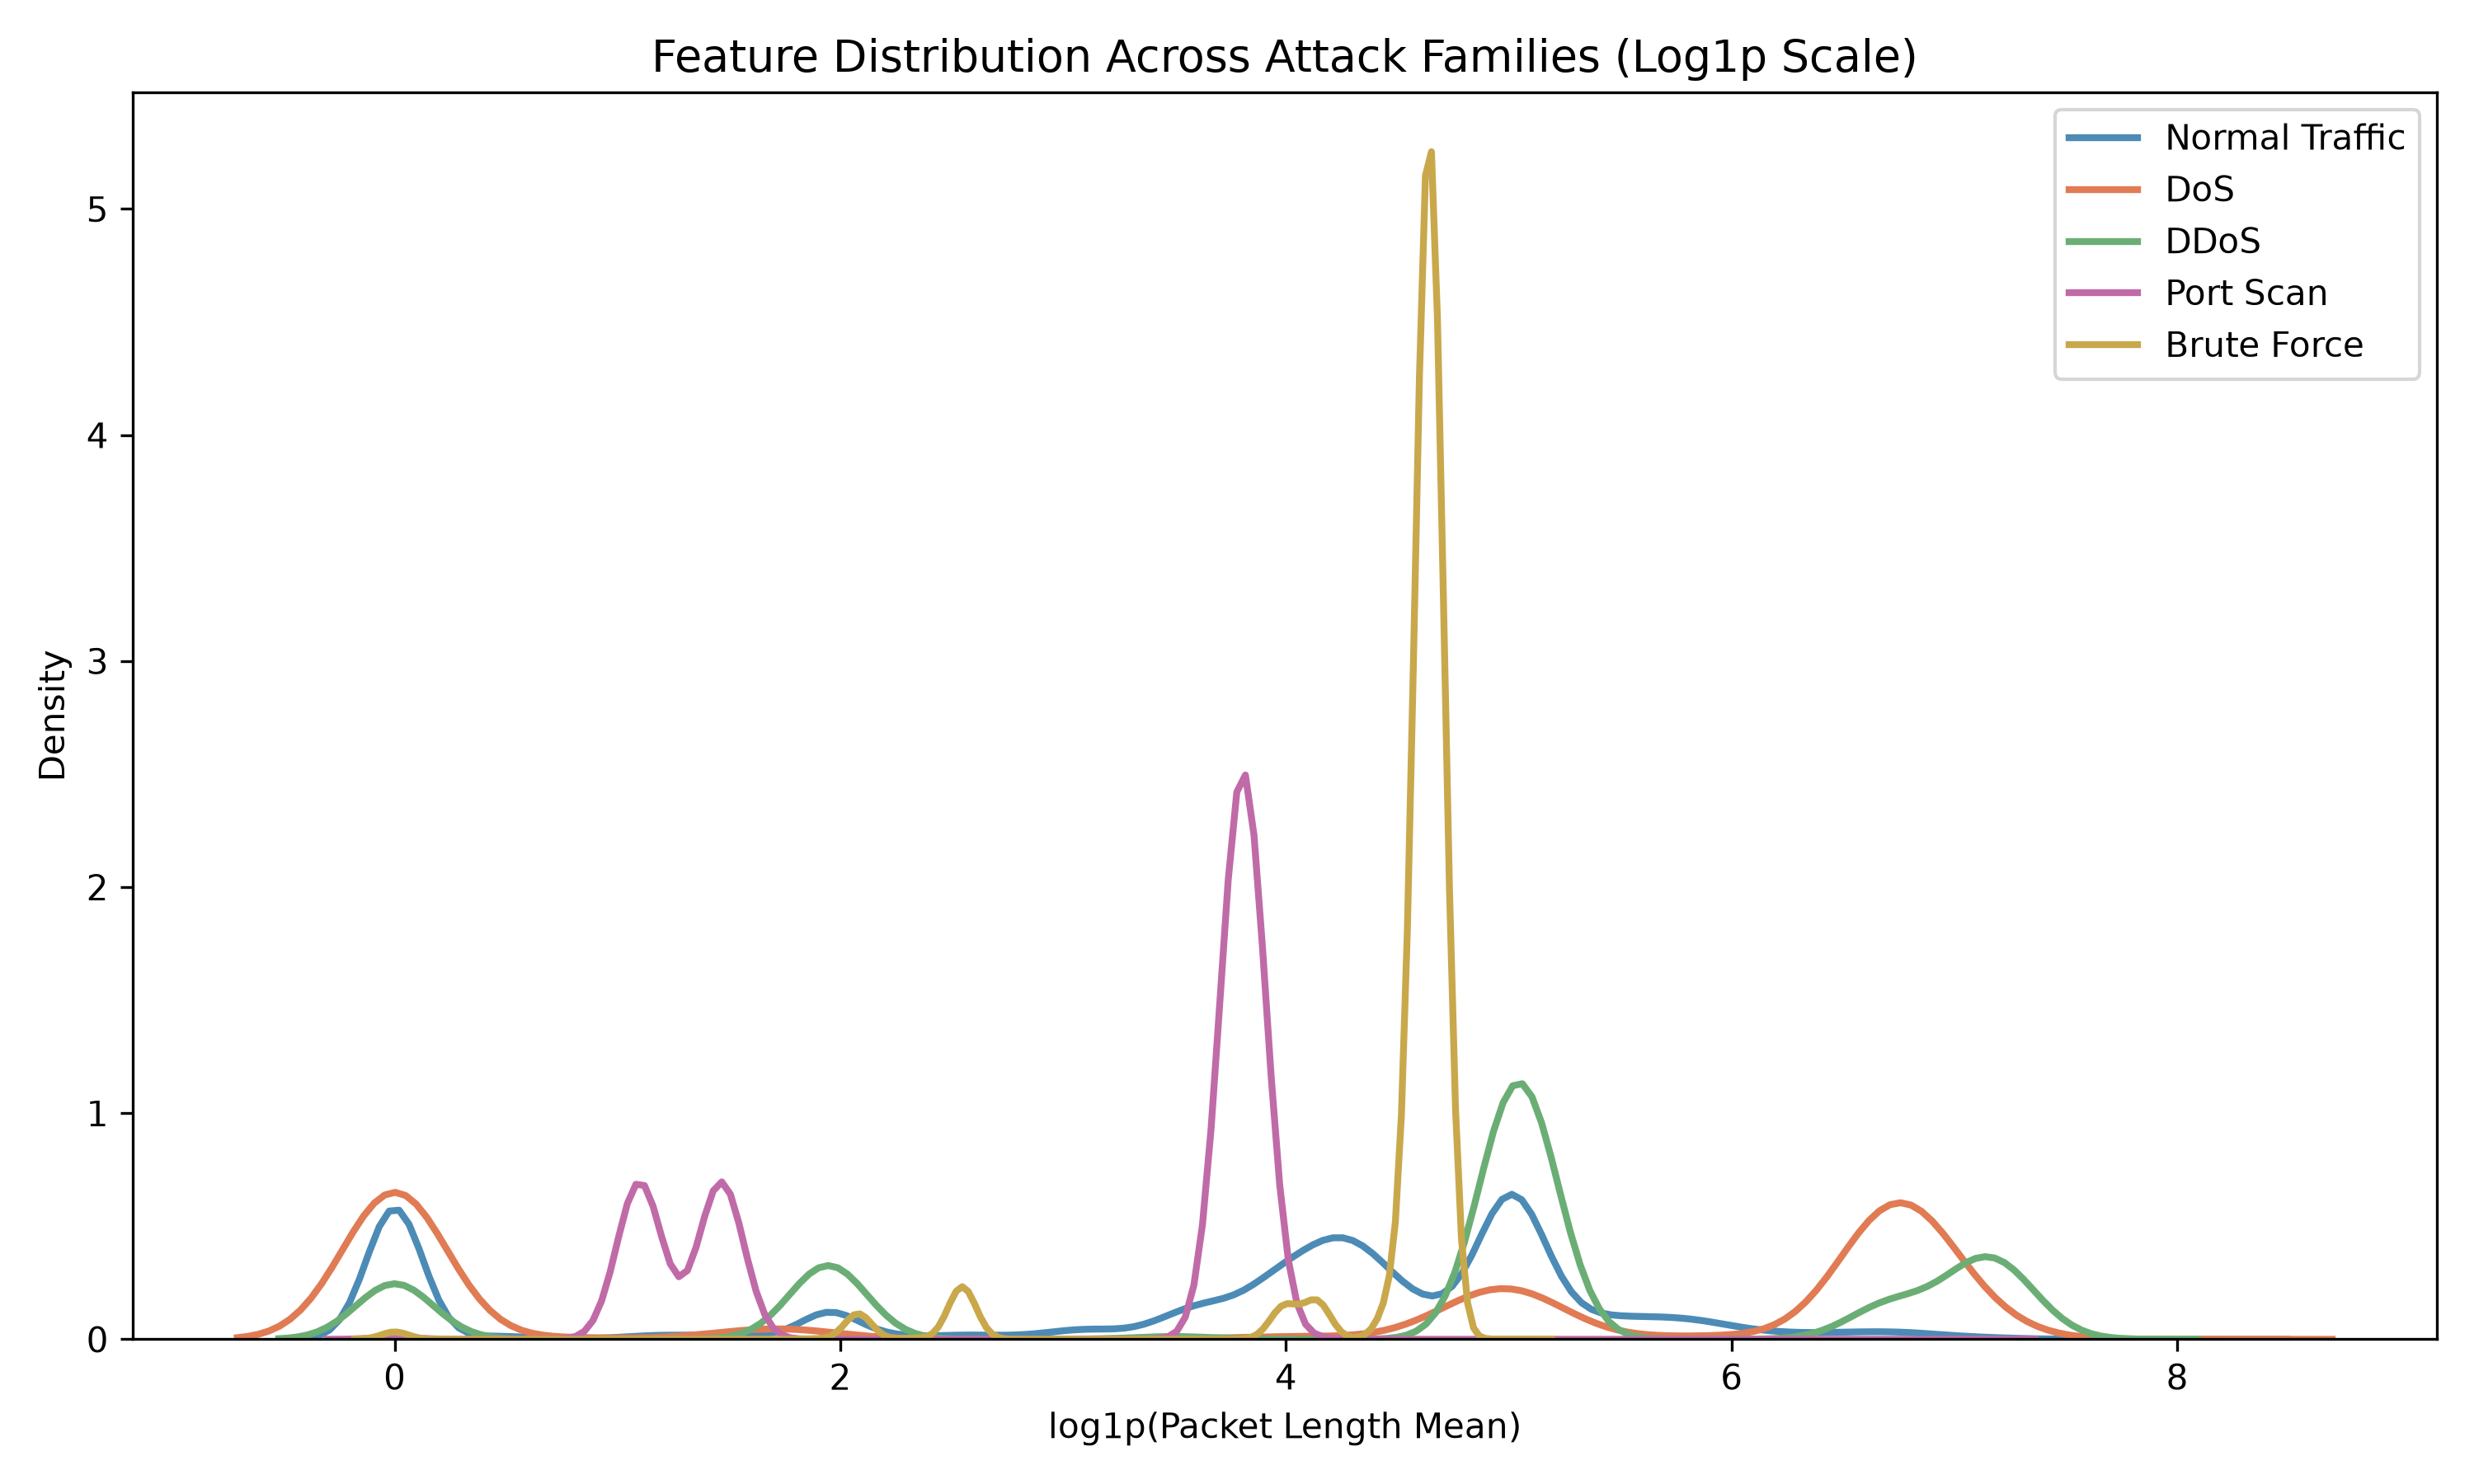
\includegraphics[width=0.85\textwidth]{fig3_1_feature_distribution.png}
\caption{Feature Distribution Across Attack Families (Log1p Scale)}
\label{fig:feat_dist}
\end{figure}

Visualizing the features on a logarithmic scale, as shown in Figure~\ref{fig:feat_dist}, reveals distinct behavioral patterns across different attack categories. Packet Length Mean shows strong class separation: Port Scan traffic produces an extremely sharp, narrow spike at very low values, consistent with its near-zero mean packet length of 3.25 bytes. DDoS traffic concentrates at a high value with a tight distribution, reflecting its mean of 736.9 bytes. DoS is similarly elevated at 565.7 bytes but more spread out. Normal Traffic and Brute Force overlap considerably in the mid-range.

Flow Duration shows the clearest separation for Port Scan, which produces a sharp isolated spike at very low durations (mean 82,820 $\mu$s), consistent with rapid probe-style connections. DoS flows have the longest durations (mean $5.57 \times 10^7$ $\mu$s), forming a distinct cluster at the high end.

While certain attack classes exhibit highly specific, isolated signatures in individual features, substantial overlap exists between Normal Traffic and attack classes across the lower ranges of most features. No single feature provides a clean decision boundary across all five classes. This analysis supports the use of a multi-feature, non-linear ensemble approach capable of exploiting the combined discriminative signal across all 40 selected features.

\section{Data Visualization}

\begin{figure}[H]
\centering
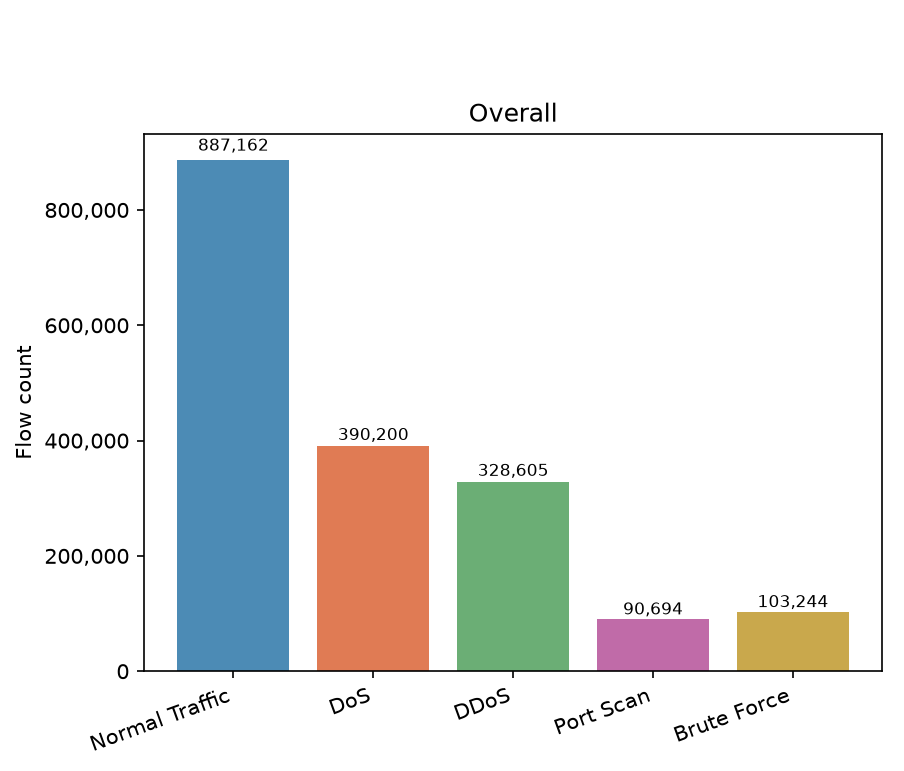
\includegraphics[width=0.65\textwidth]{class_distribution.png}
\caption{Class Distribution}
\label{fig:class_dist}
\end{figure}

Figure~\ref{fig:class_dist} illustrates the class distribution of the curated 1,799,905-flow benchmark. Following the 15\% subsampling of benign records, Normal Traffic represents 49.3\% of the corpus (887,162 flows), while DoS (21.7\%, 390,200 flows) and DDoS (18.3\%, 328,605 flows) constitute the primary attack vectors. The minority attack classes, Brute Force (5.7\%, 103,244 flows) and Port Scan (5.0\%, 90,694 flows), maintain substantial absolute sample counts sufficient to train deep decision boundaries without severe minority underfitting.

\begin{figure}[H]
\centering
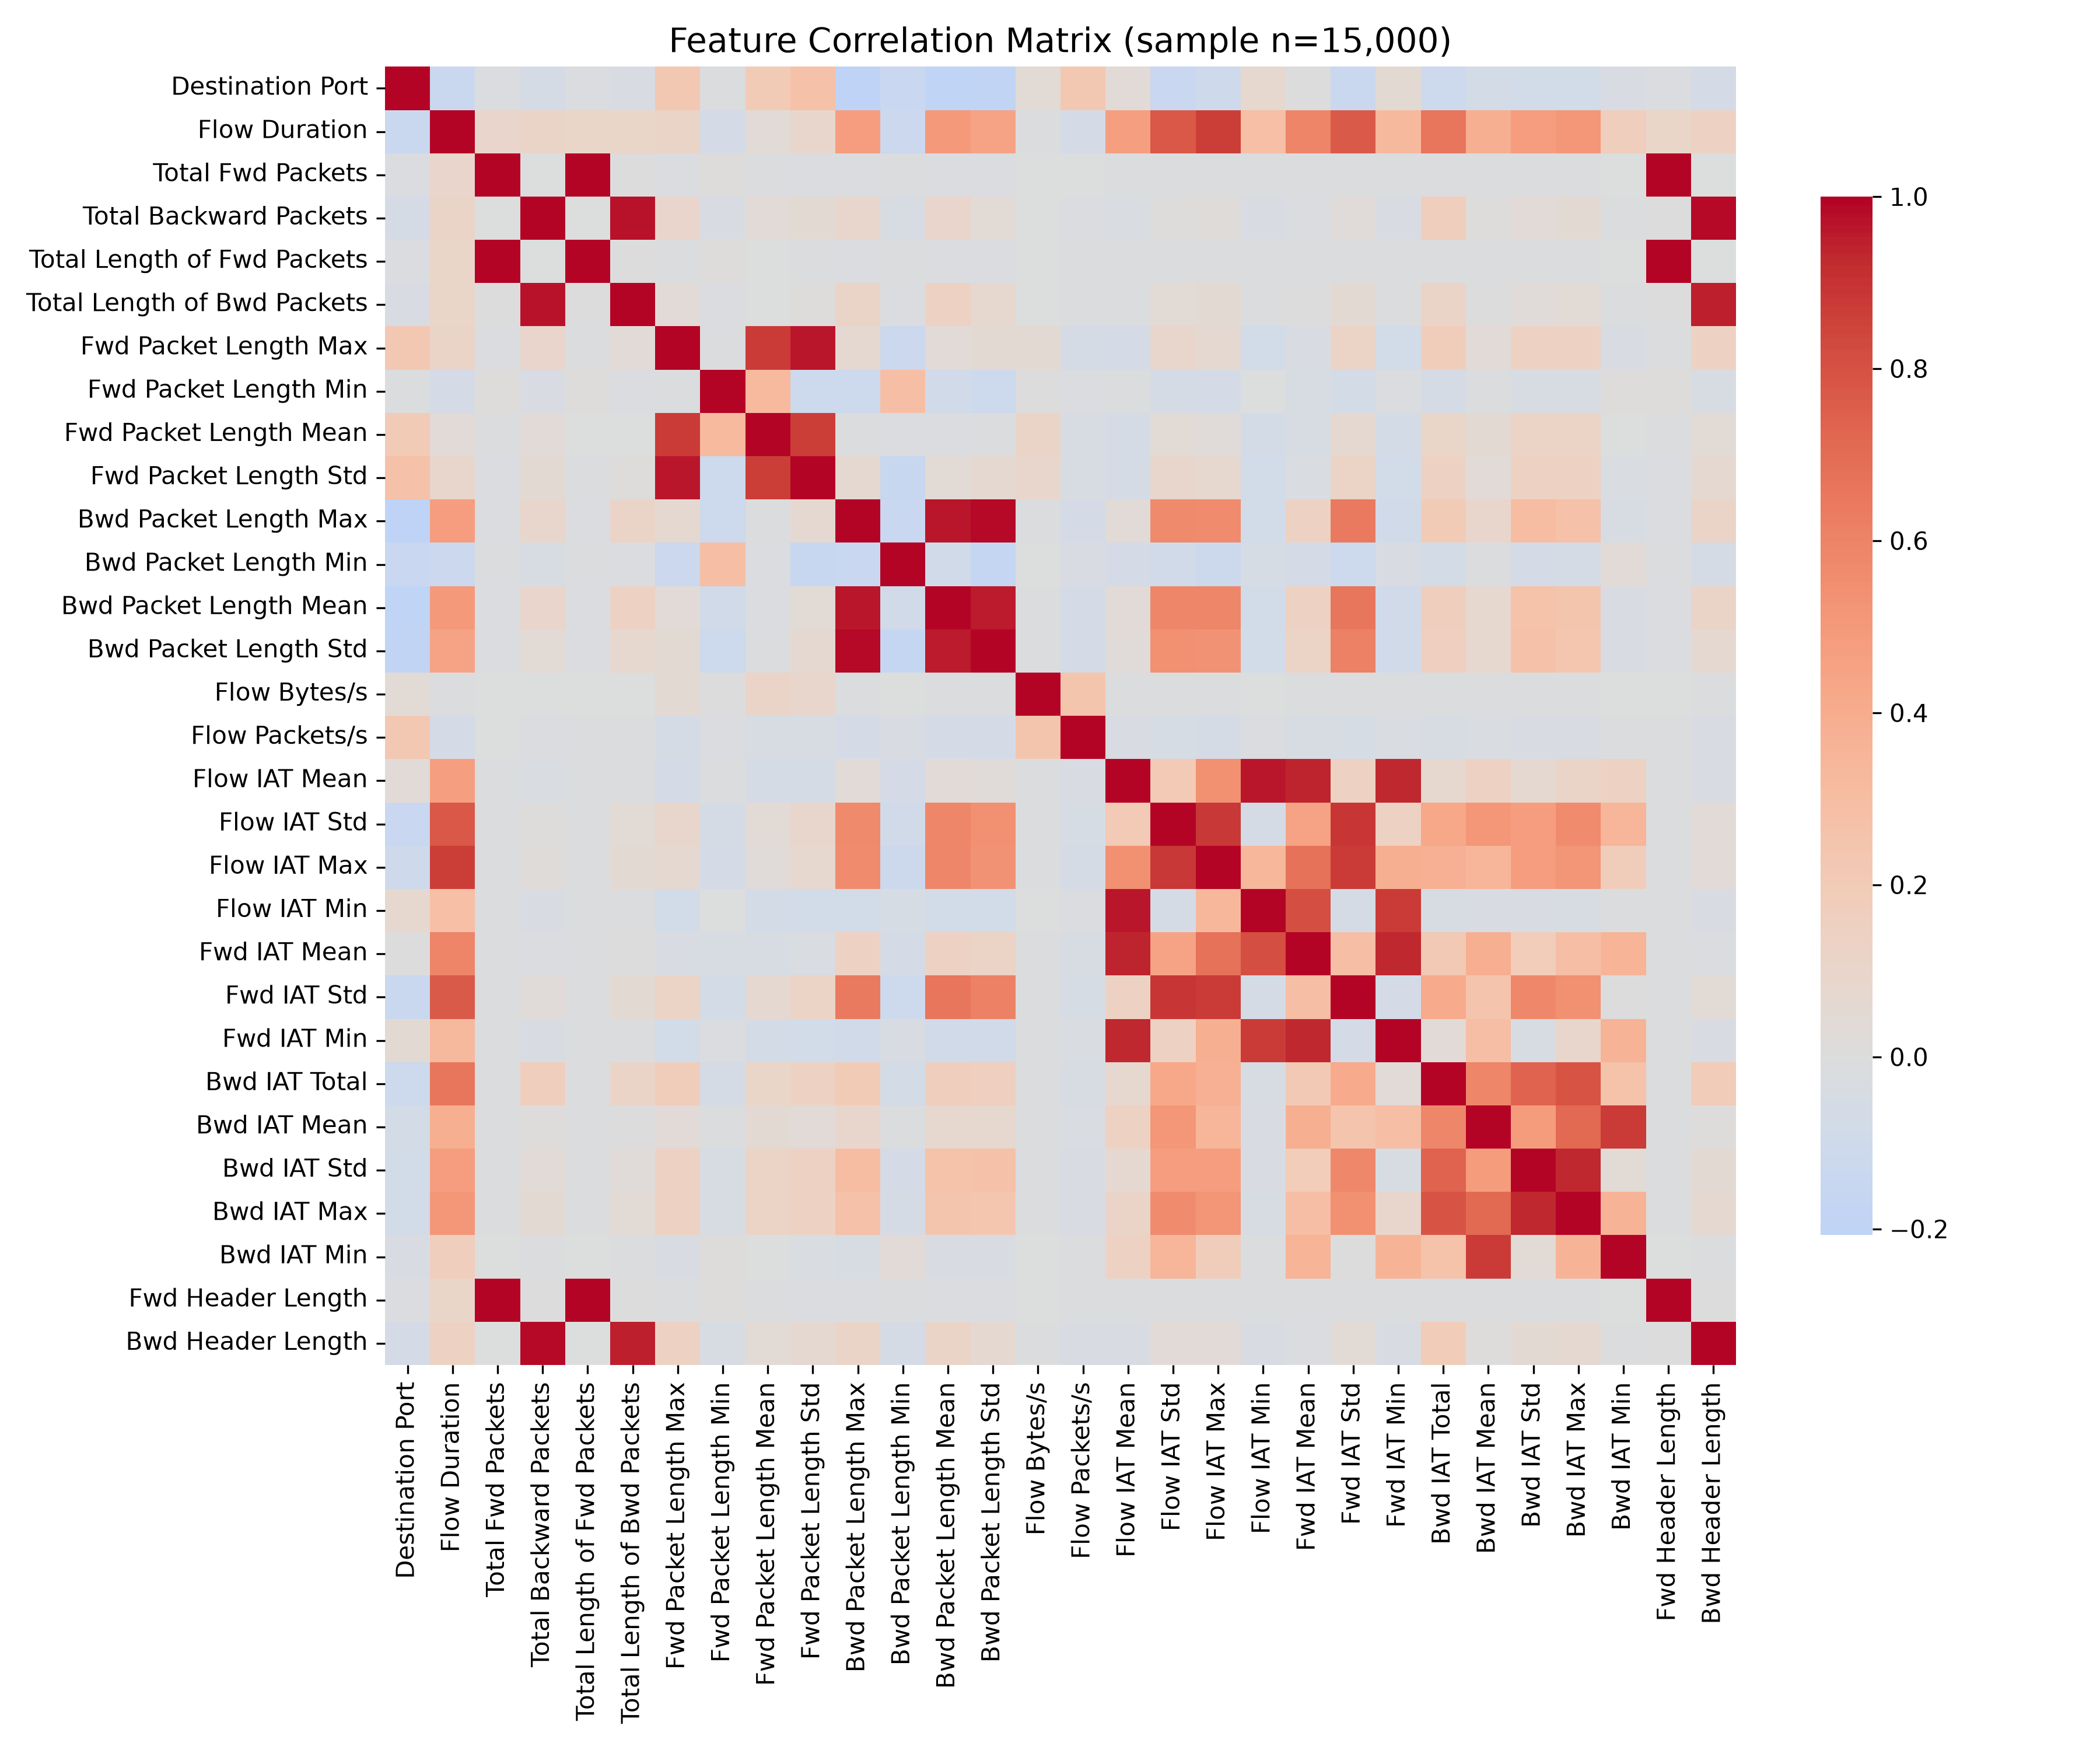
\includegraphics[width=0.75\textwidth]{fig3_3_correlation_matrix.png}
\caption{Feature Correlation Matrix (sample n=15,000)}
\label{fig:corr_matrix}
\end{figure}

Figure~\ref{fig:corr_matrix} displays the Pearson correlation matrix computed on a random sample of 15,000 records across the full feature set. The heatmap reveals several distinct clusters of high redundancy, with 27 feature pairs exceeding a correlation threshold of 0.99. The most striking redundancies are perfect correlations ($r = 1.0000$): Total Fwd Packets with Subflow Fwd Packets, Total Backward Packets with Subflow Bwd Packets, Total Length of Fwd Packets with Subflow Fwd Bytes, Fwd Packet Length Mean with Avg Fwd Segment Size, Bwd Packet Length Mean with Avg Bwd Segment Size, and Fwd Header Length with Fwd Header Length.1. These findings directly informed the correlation-based feature reduction step in the preprocessing pipeline, reducing the feature set from 69 to 53 features prior to statistical, importance-based, and domain-refinement selection.

\begin{figure}[H]
\centering
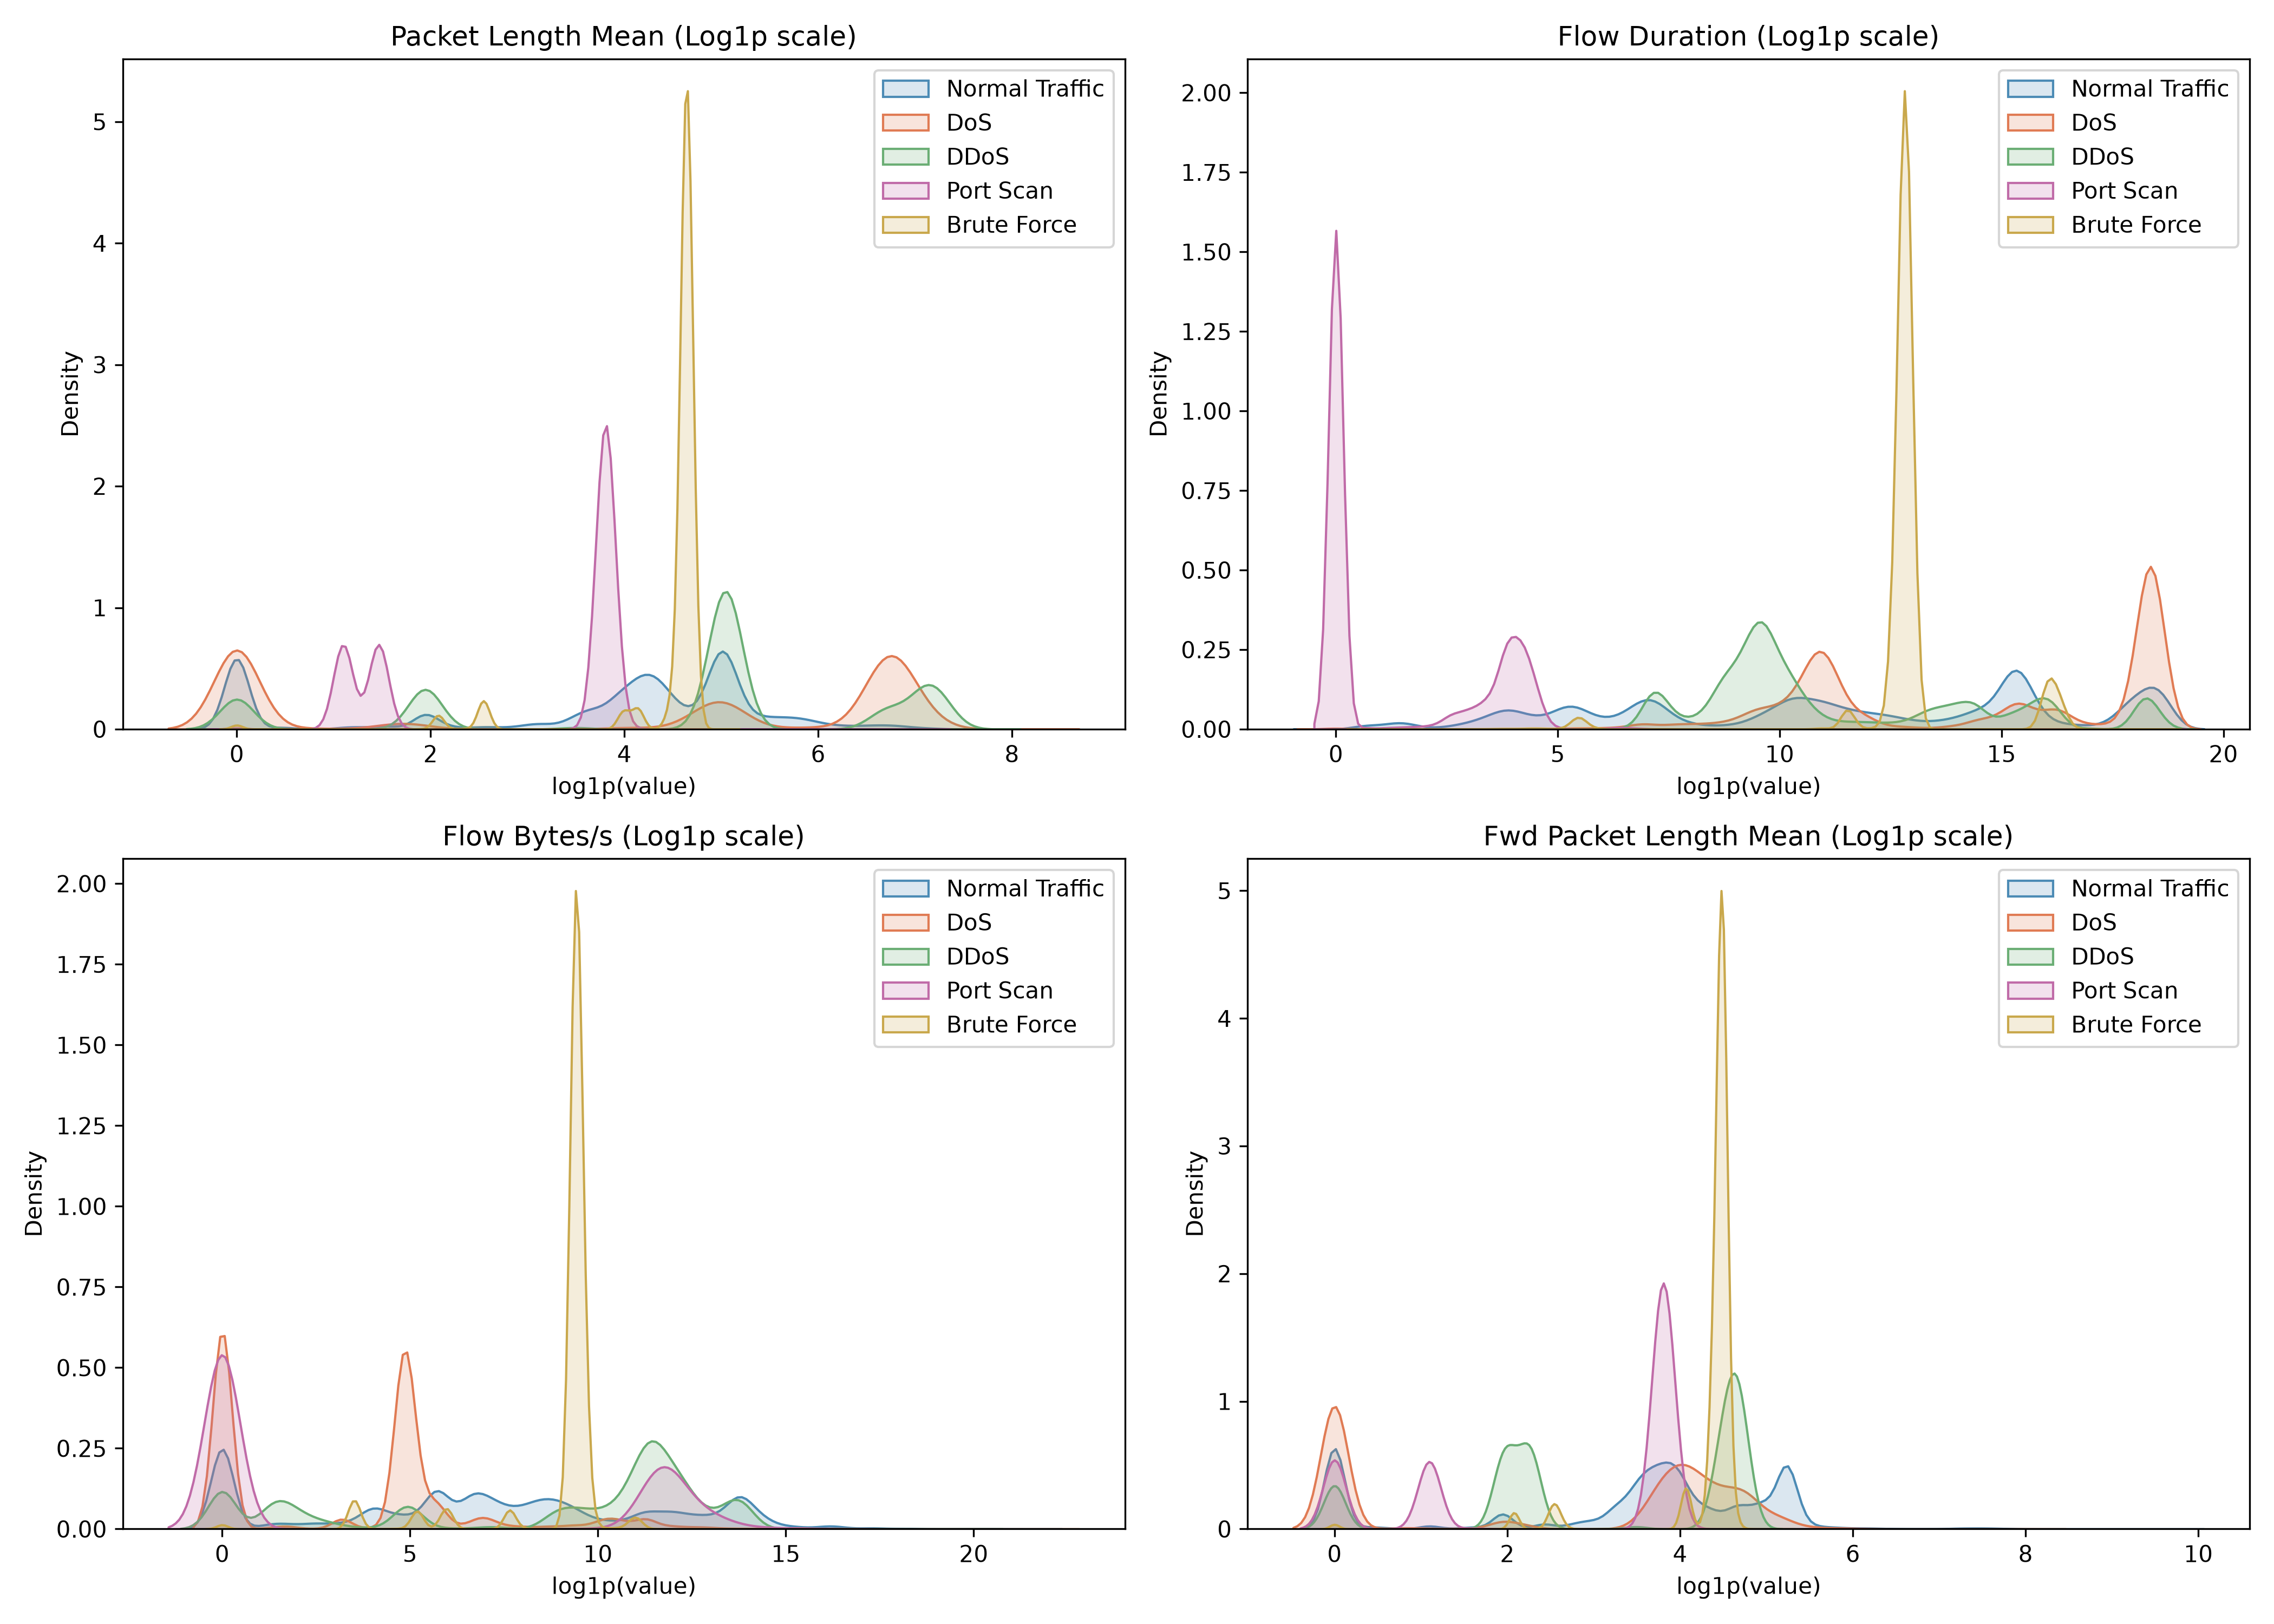
\includegraphics[width=0.9\textwidth]{fig3_4_key_feature_distributions.png}
\caption{Key Feature Distributions by Attack Type}
\label{fig:key_feat_dist}
\end{figure}

Figure~\ref{fig:key_feat_dist} shows the density distributions of four key features, Packet Length Mean, Flow Duration, Flow Bytes/s, and Fwd Packet Length Mean, stratified by the five attack classes on a log1p scale. Across all four features, the distributions are heavily right-skewed, with most values concentrated near zero and long tails extending toward high values. Port Scan produces a sharp, isolated spike at very low Packet Length Mean values, while DDoS and DoS cluster at higher values with tighter distributions. Flow Duration shows Port Scan concentrated at very short durations, consistent with rapid probe-style connections, while DoS spans the highest duration range, reflecting sustained flooding behaviour. Flow Bytes/s reveals a distinctive high-value spike for Port Scan, while DoS shows a prominent mid-range concentration and Normal Traffic spreads broadly across lower values. Fwd Packet Length Mean shows the sharpest class separation, with Brute Force and DDoS producing extremely narrow, high-density spikes at low values, clearly distinguishable from the broader Normal Traffic distribution. The visible separation between classes across these features confirms their relevance as discriminative inputs to the ensemble classifier.

\begin{figure}[H]
\centering
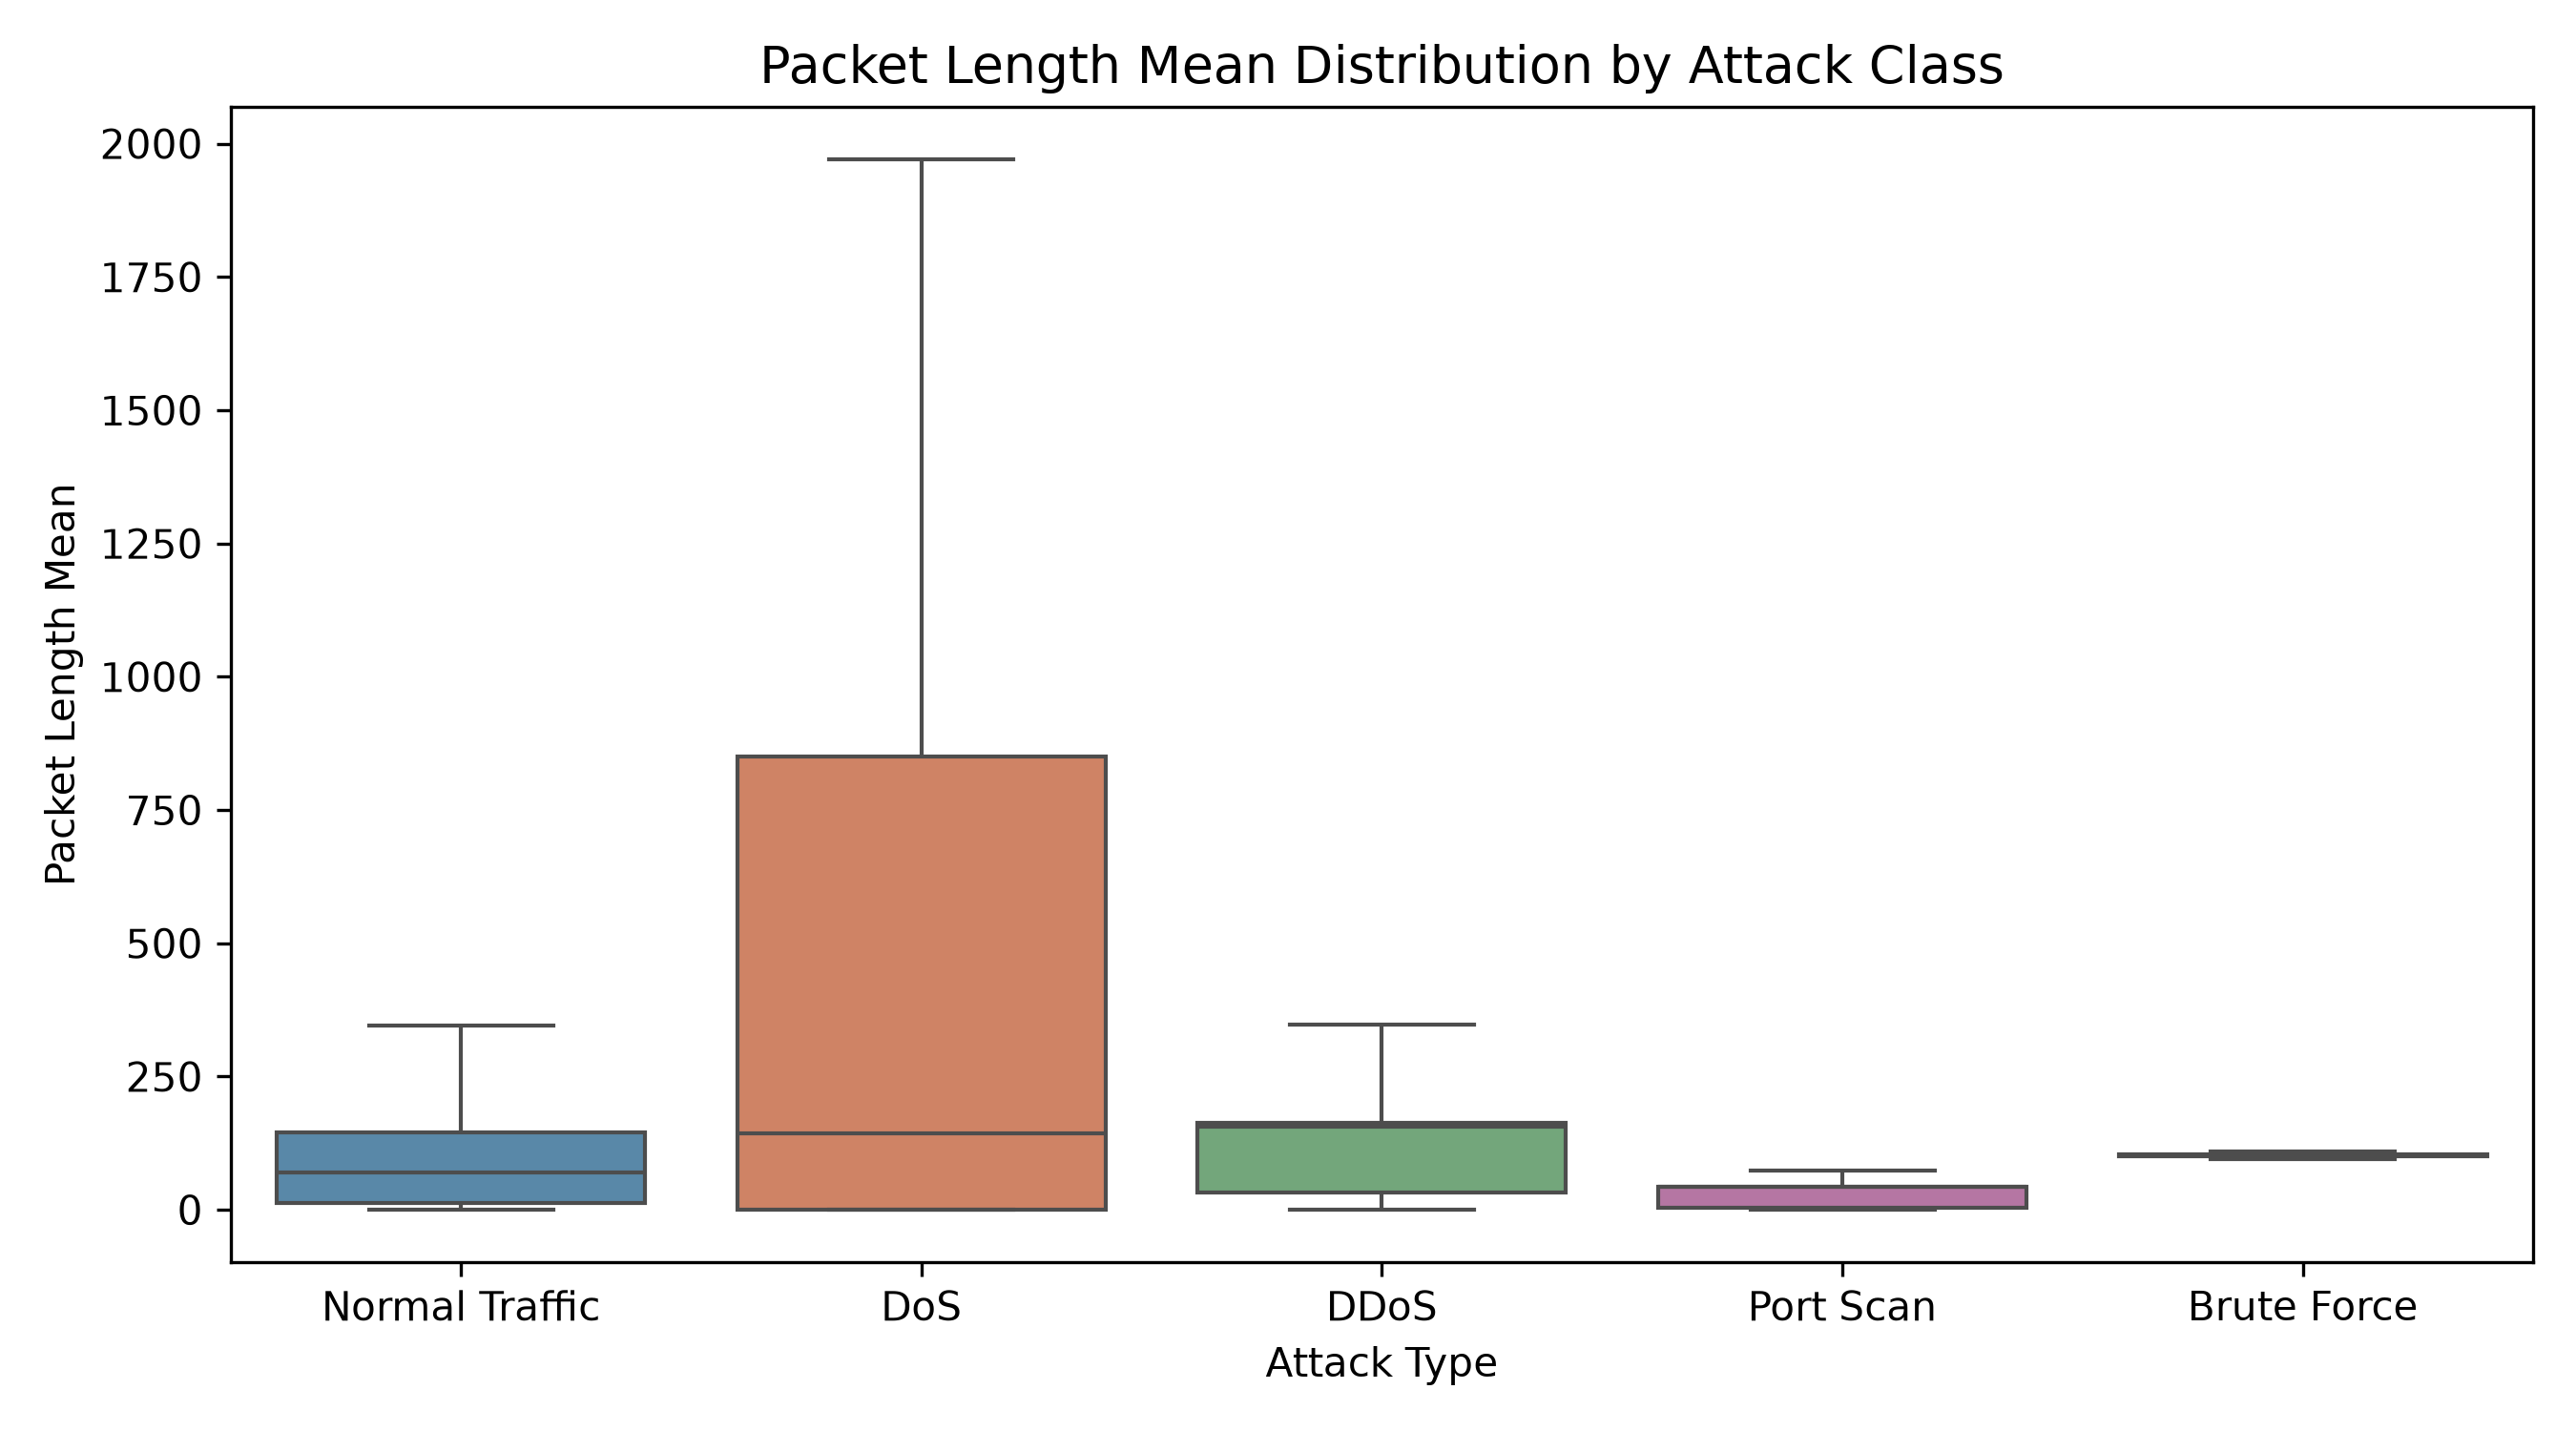
\includegraphics[width=0.85\textwidth]{fig3_5_packet_length_mean_boxplot.png}
\caption{Packet Length Mean Distribution by Attack Class}
\label{fig:packet_len_dist}
\end{figure}

Figure~\ref{fig:packet_len_dist} presents box plots of Packet Length Mean across the five traffic classes. DDoS and DoS show substantially higher median packet lengths, approximately 800 bytes each, with DDoS exhibiting a wider interquartile range indicating greater variability in payload size. Normal Traffic has a low median of approximately 80 bytes with a moderate spread. Port Scan and Brute Force both have medians near zero, consistent with the short probe packets characteristic of scanning activity and the small credential packets used in brute force attempts. These inter-class differences in packet length make it a strongly discriminating feature for the ensemble model, as confirmed by its top-10 ranking in Random Forest feature importance.

\begin{figure}[H]
\centering
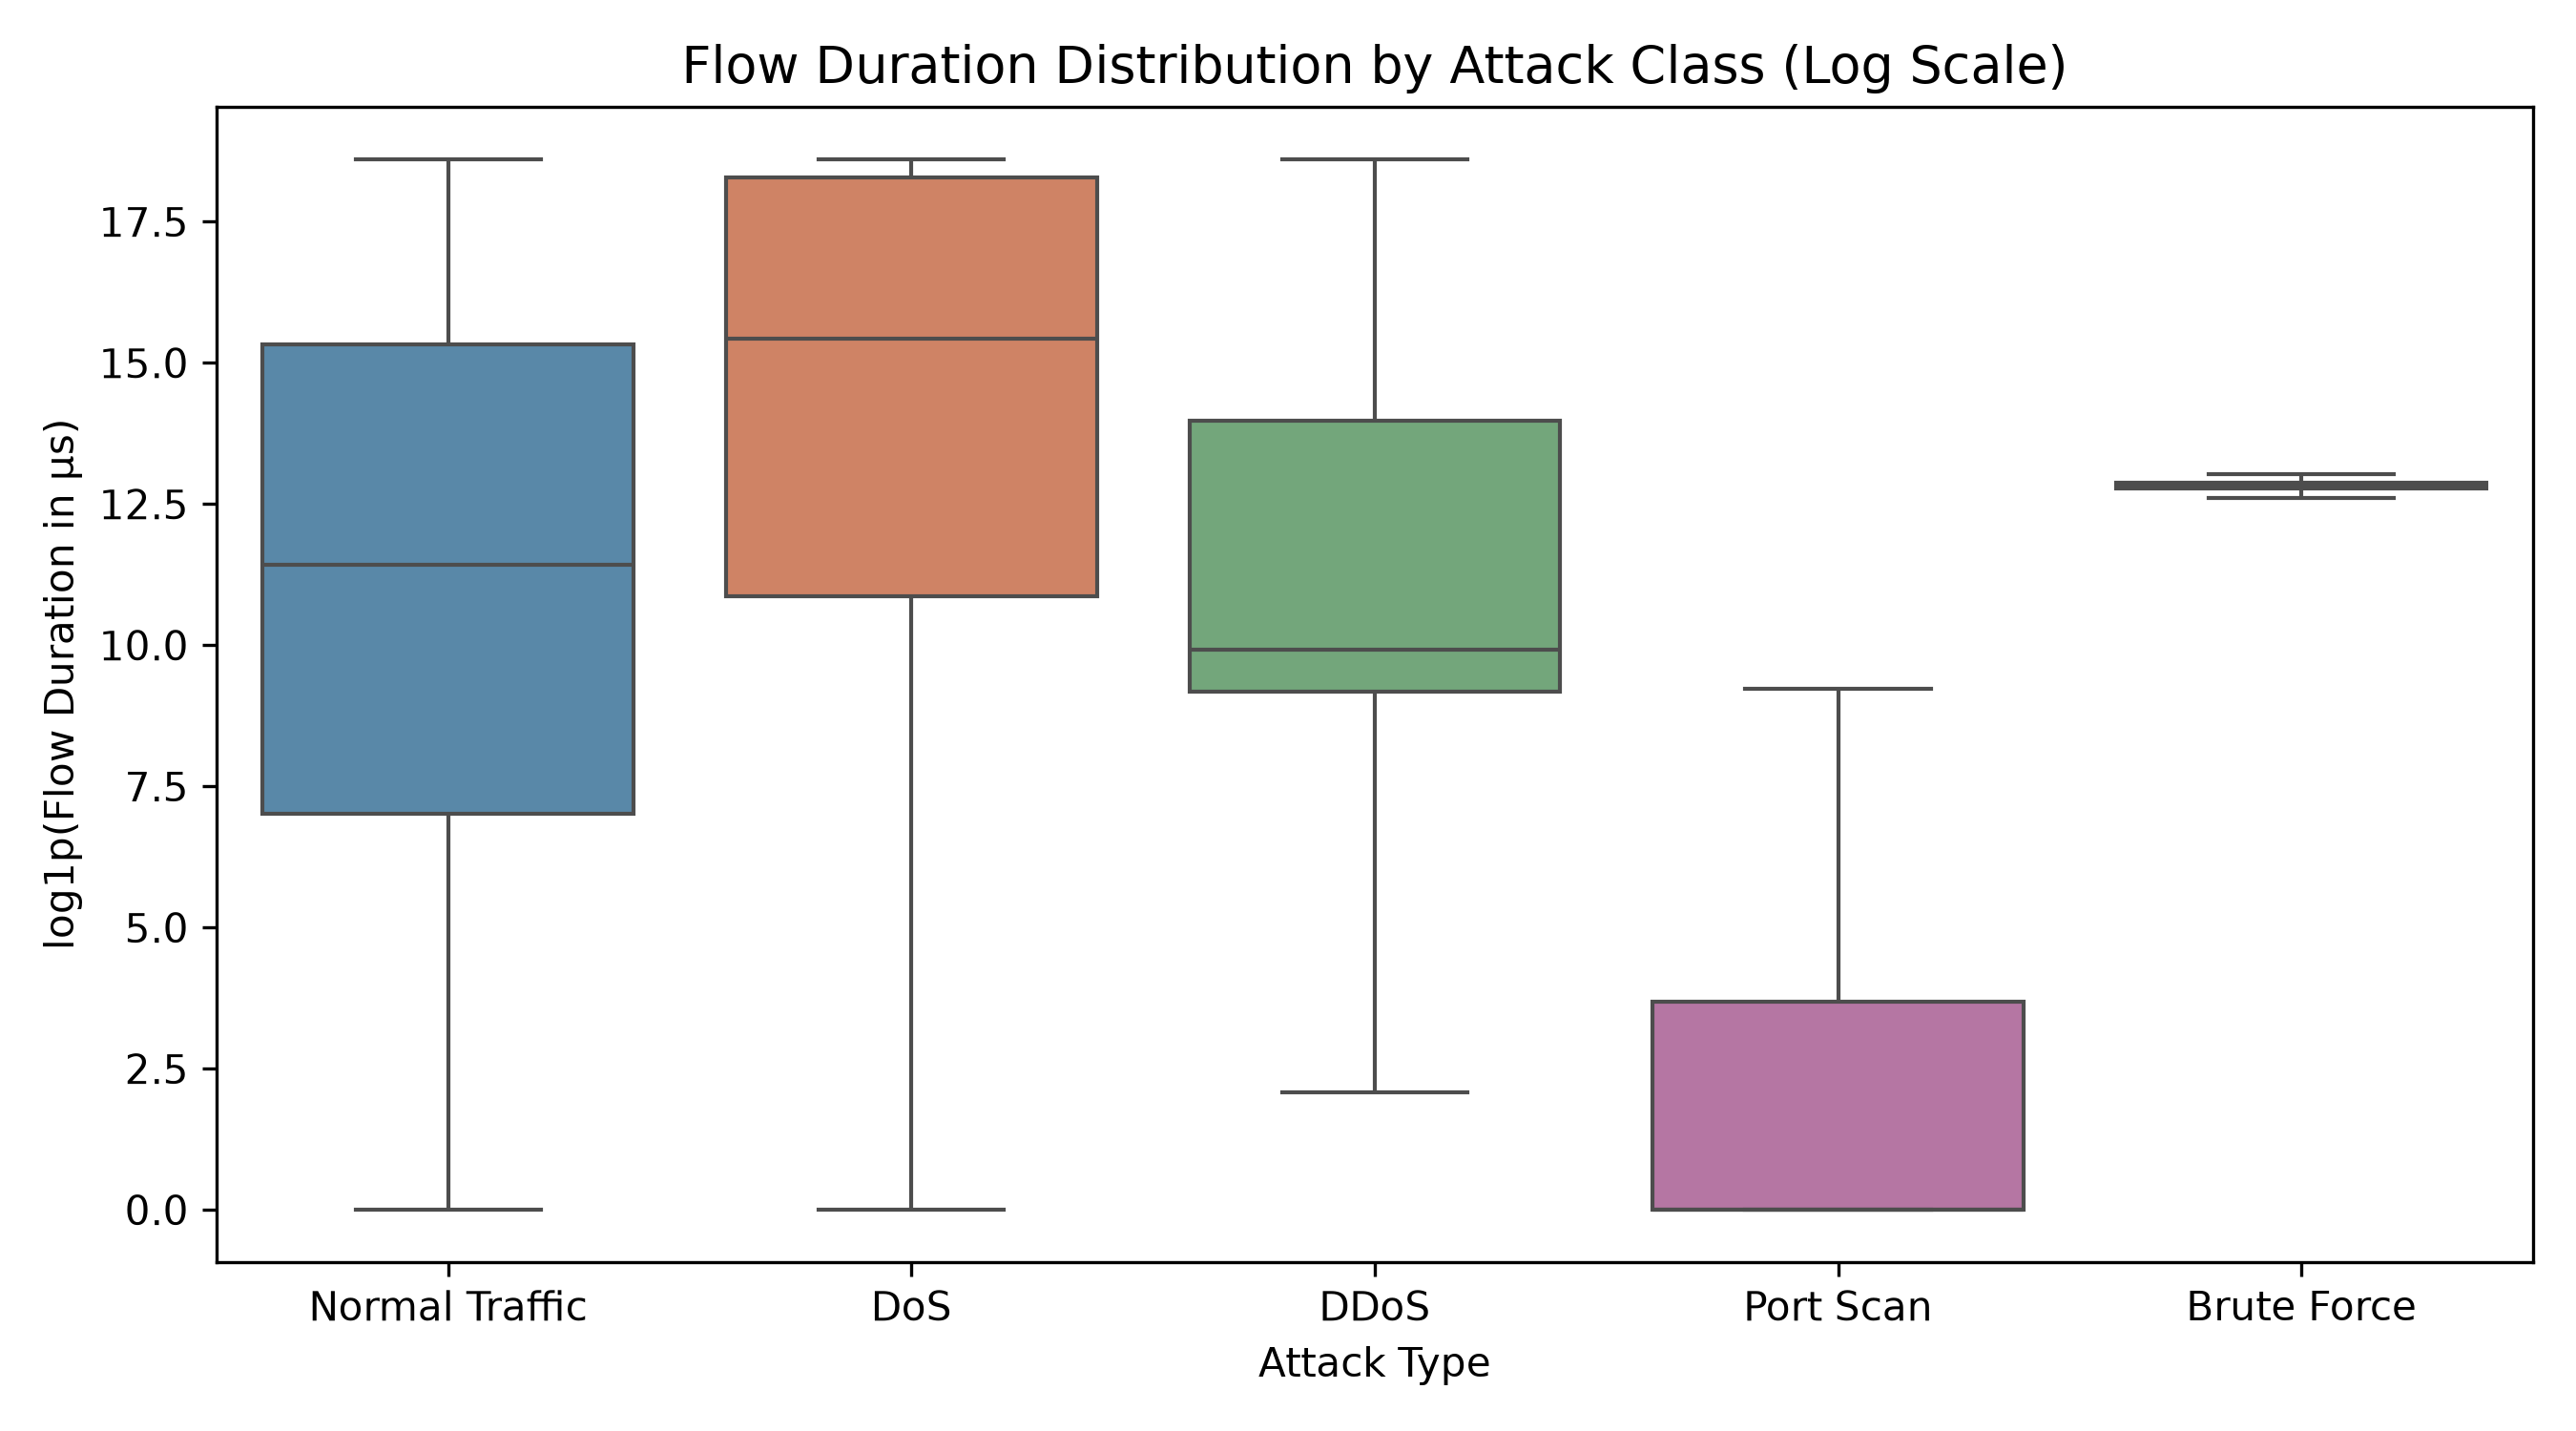
\includegraphics[width=0.85\textwidth]{fig3_6_flow_duration_boxplot.png}
\caption{Flow Duration Distribution by Attack Class (Log Scale)}
\label{fig:flow_dur_dist}
\end{figure}

Figure~\ref{fig:flow_dur_dist} shows box plots of Flow Duration on a log1p scale across the five traffic classes. DoS flows exhibit by far the longest durations, consistent with sustained flooding behaviour that keeps connections open for extended periods. DDoS, Brute Force, and Normal Traffic all have low medians compressed near zero relative to DoS, though with varying spreads. Port Scan shows the shortest and most tightly concentrated durations, corresponding to its rapid, probe-style connection pattern. Flow Duration thus provides strong discriminative signal, particularly for separating DoS from all other classes.

\section{Analysis of Architecture and Algorithms}

\subsection{Detailed Study Report of the Proposed Algorithms}

\subsubsection*{Random Forest}

Random Forest is an ensemble learning method that constructs a large number of decision trees during training and outputs the class with the highest aggregated vote (for classification) across all trees. Each tree is trained on a bootstrap sample of the training data, and at each split, only a random subset of features is considered as candidates for the split criterion. This combination of data bagging and feature randomization reduces the variance of the ensemble compared to any individual tree and makes the model robust to overfitting, even on high-dimensional datasets such as the unified benchmark with 40 features.

Strengths: handles mixed feature scales without requiring normalization; naturally produces feature importance scores; robust to noisy or redundant features; scales efficiently to large datasets via parallel tree construction (\texttt{n\_jobs=-1}).

Justification: Ness et al.\ (2025), in a multi-model comparison on network traffic anomaly detection, demonstrated that tree-based ensemble methods consistently outperform single-model classifiers on structured network flow data. Fathima et al.\ (2024) validate their hybrid detection framework on the CIC-IDS2017 dataset, the same benchmark used here, directly supporting Random Forest's inclusion as a base learner.

\begin{figure}[H]
\centering
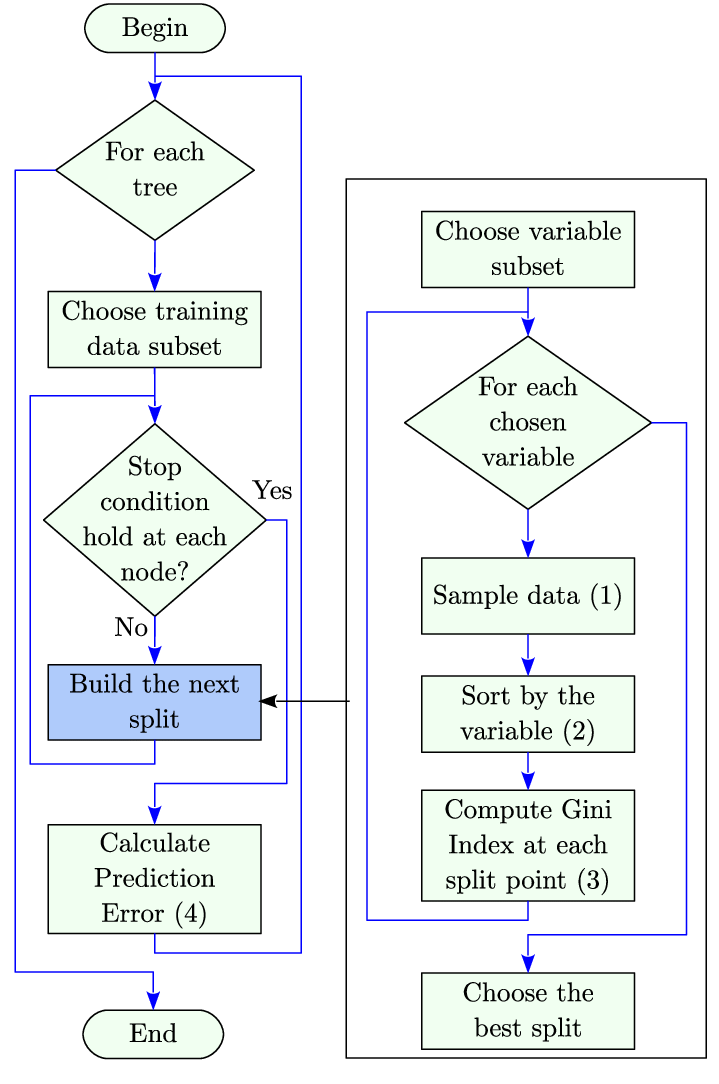
\includegraphics[width=0.55\textwidth]{image7.png}
\caption{Flowchart of Random Forest}
\label{fig:rf_flowchart}
\end{figure}

\subsubsection*{XGBoost}

Extreme Gradient Boosting (XGBoost) is a gradient boosting framework that builds an ensemble of decision trees sequentially, where each successive tree is trained to correct the residual errors of the previous ensemble. Unlike Random Forest, which builds trees independently in parallel, XGBoost applies a gradient descent optimization procedure in function space, minimizing a regularized loss function at each step. L1 and L2 regularization terms in its objective function additionally control overfitting.

Strengths: superior performance on structured/tabular data due to boosting-based bias reduction; built-in regularization; supports GPU-accelerated training via \texttt{tree\_method='hist'}; native handling of multi-class classification via softmax objective (\texttt{eval\_metric='mlogloss'}).

Justification: Ness et al.\ (2025) evaluated XGBoost directly against four other models on network traffic anomaly detection, finding it among the strongest individual classifiers with a test accuracy of 0.83 and F1-score of 0.84. Ji C et al.\ (2025), evaluated on the same CIC-IDS2017 dataset, provide a direct performance reference point: their GRU-ResCBANet model achieved 99.79\% multi-class accuracy, against which the ensemble's results can be situated.

\begin{figure}[H]
\centering
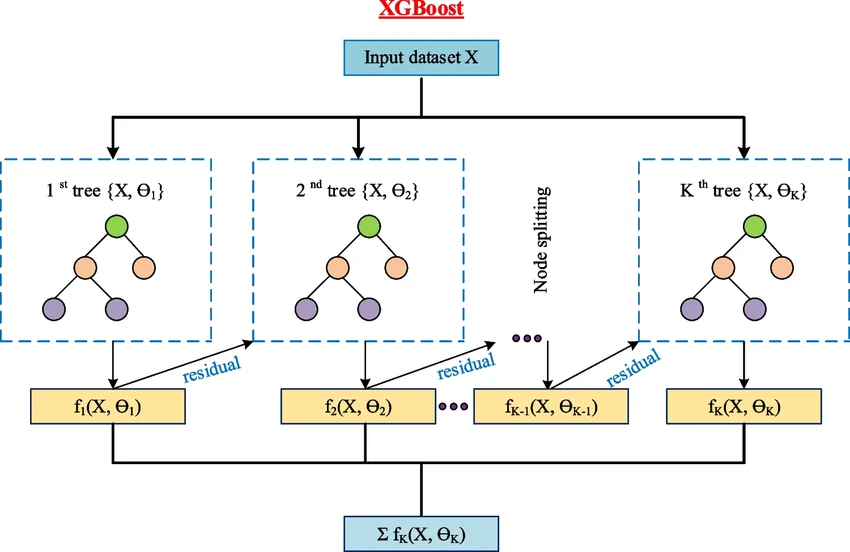
\includegraphics[width=0.75\textwidth]{image8.png}
\caption{Flowchart of XGBoost}
\label{fig:xgb_flowchart}
\end{figure}

\subsubsection*{Soft-Voting Ensemble}

The proposed system combines Random Forest and XGBoost in a soft-voting ensemble. In soft voting, each base model outputs a probability distribution over the five classes for each input flow. The ensemble averages these probability vectors across both models, and the class with the highest average probability is selected as the final prediction. This approach leverages the calibrated confidence of each model: when both models agree, the ensemble prediction is strongly reinforced; when they disagree, the aggregated probability distributes confidence appropriately, reducing the risk of a single model's error driving the final output.

Strengths: combines complementary inductive biases (RF's variance reduction through bagging with XGBoost's bias reduction through boosting); soft probability averaging suppresses individual model errors and reduces false positives, directly addressing the primary reliability concern in operational IDS deployment.

Justification: Fathima et al.\ (2024) demonstrate that high false positive rates are the central practical failure mode of IDS systems. Ensemble soft voting directly addresses this by averaging probability vectors, pulling inflated attack probability predictions back toward the correct class. Ji C et al.\ (2025) provide a direct benchmark on intrusion detection: their deep learning hybrid architecture achieves 99.79\% multi-class accuracy, while the proposed RF + XGBoost soft-voting ensemble achieves 99.94\% accuracy on the combined benchmark, confirming that the ensemble is highly competitive with architecturally complex deep models.

\section{Project Pipeline}

\subsection{Project Pipeline Diagram and Development Plan}

The NIDAS system is organised into seven functional stages, from raw traffic acquisition through to real-time alert generation and output delivery. Figure~\ref{fig:pipeline} illustrates the complete end-to-end architecture:

\begin{figure}[H]
\centering
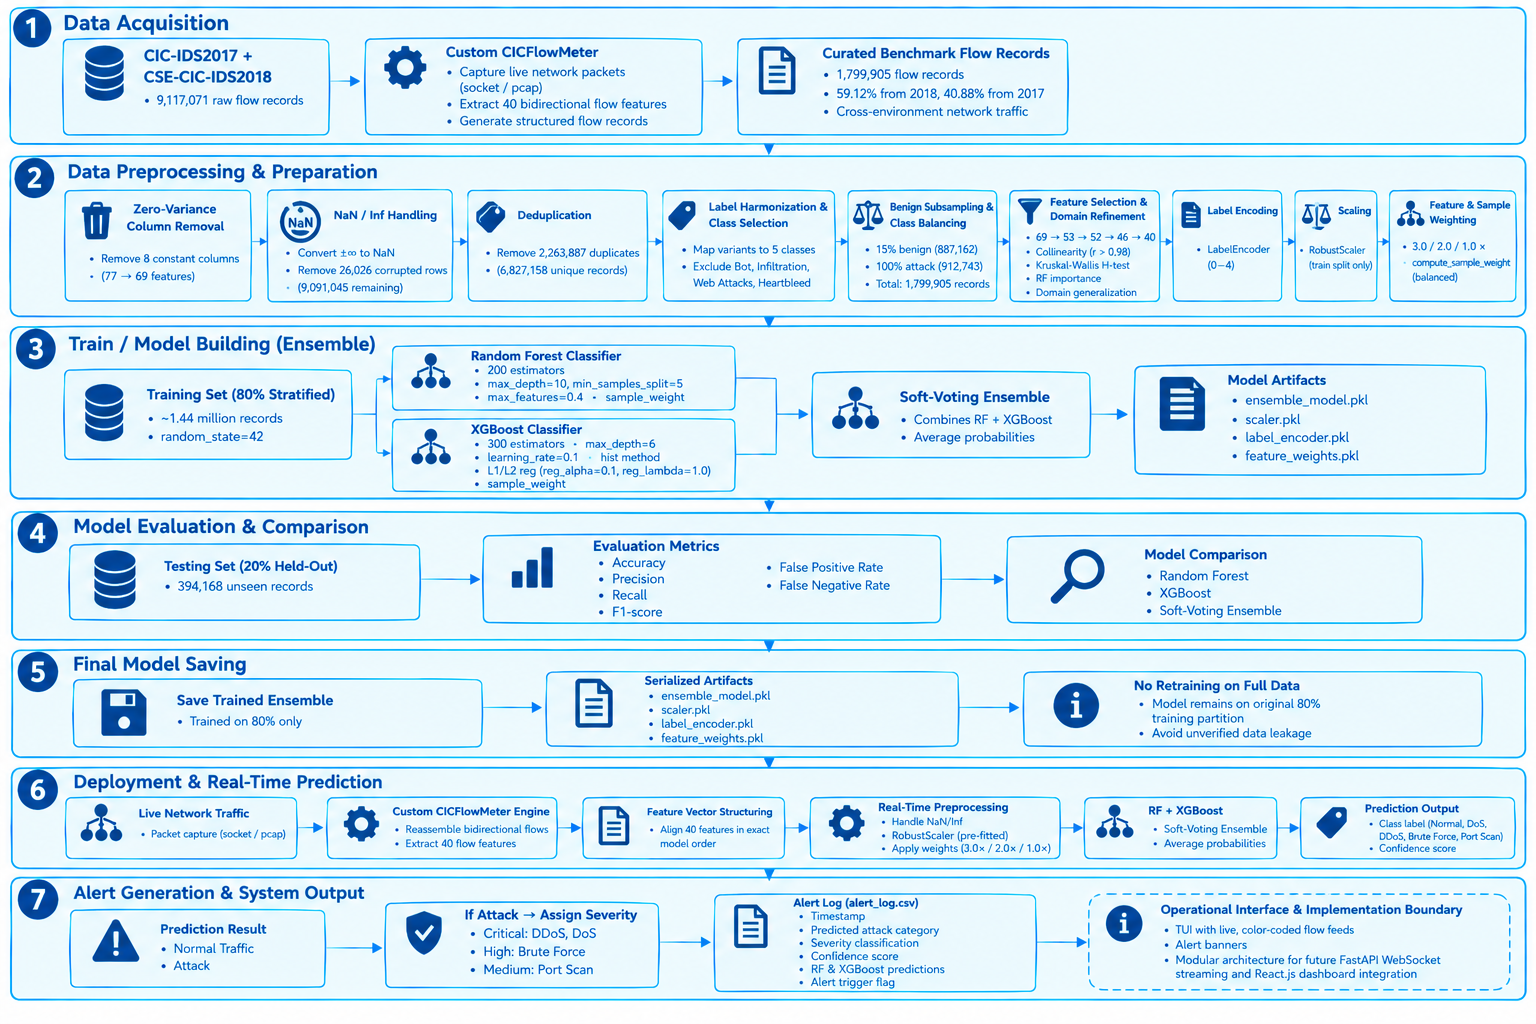
\includegraphics[width=0.95\textwidth]{pipeline.png}
\caption{Project Pipeline}
\label{fig:pipeline}
\end{figure}

\begin{enumerate}[leftmargin=*]
    \item \textbf{Data Acquisition:} The system integrates 9,117,071 raw flow records from the CIC-IDS2017 and CSE-CIC-IDS2018 benchmarks, capturing 77 initial numeric flow characteristics and target metadata. After deduplication, cleaning, and subsampling, a curated benchmark of 1,799,905 flow records is established (59.12\% from 2018 and 40.88\% from 2017) to provide robust multi-environment representation. In deployment, a custom Python CICFlowMeter engine captures live packets from network sockets/PCAP and extracts the identical 40 bidirectional flow features in real time.
    
    \item \textbf{Data Preprocessing and Preparation:} The raw corpus undergoes zero-variance removal (dropping 8 constant features, reducing 77 to 69 dimensions), conversion of $\pm\infty$ values to NaN and dropping of 26,026 corrupted rows, and deduplication of 2,263,887 duplicate records. Labels are harmonized into five core classes (Normal Traffic, DoS, DDoS, Brute Force, and Port Scan) while peripheral attack classes are excluded. Benign records are subsampled at 15\% (887,162 flows) and merged with 100\% of attack records. A four-stage feature refinement process ($69 \rightarrow 53 \rightarrow 52 \rightarrow 46 \rightarrow 40$) eliminates collinear and domain-sensitive features. Categorical labels are encoded using \texttt{LabelEncoder} ($0$--$4$), inputs are normalized using \texttt{RobustScaler} fitted exclusively on the training split, and discriminative feature weights ($3.0\times$, $2.0\times$, $1.0\times$) and balanced sample weights are computed.
    
    \item \textbf{Train / Model Building (Ensemble):} An 80\% stratified training partition ($\approx 1.44$ million flows) is used to train the base estimators. Random Forest (200 trees, \texttt{max\_depth=10}, \texttt{max\_features=0.4}) and XGBoost (300 estimators, \texttt{max\_depth=6}, \texttt{learning\_rate=0.1}, GPU histogram method) are fitted independently using the precomputed balanced sample weights on the weighted feature space. The soft-voting ensemble is constructed by combining the pre-fitted estimators to compute probability averages across both models. Serialized model artifacts (\texttt{ensemble\_model.pkl}, \texttt{scaler.pkl}, \texttt{label\_encoder.pkl}, and \texttt{feature\_weights.pkl}) are generated.
    
    \item \textbf{Model Evaluation and Comparison:} The trained ensemble is evaluated on the held-out 20\% test partition (394,168 unseen flows). Comprehensive multi-class evaluation metrics are computed, including overall Accuracy (99.94\%), Macro F1 (0.9994), Weighted F1 (0.9994), per-class Precision, Recall, and F1-scores, as well as operational False Positive Rates (0.021\% on benign traffic) and False Negative Rates. Standalone Random Forest and XGBoost baselines are benchmarked against the soft-voting ensemble.
    
    \item \textbf{Final Model Saving:} The trained ensemble artifacts are serialized directly from the 80\% training split. To preserve empirical validity and prevent unverified data leakage, the models are not retrained on the full dataset, ensuring that all production artifacts strictly reflect the validated test partition boundaries.
    
    \item \textbf{Deployment and Real-Time Prediction:} In the operational deployment pipeline, live network traffic is captured via network sockets. The custom CICFlowMeter reassembles packets into bidirectional flows, extracts the 40 flow features, and formats them in the exact column ordering expected by the model. The real-time preprocessing stage verifies finite values, applies the pre-fitted \texttt{RobustScaler}, scales features using the discriminative weight vector, and executes soft-voting inference across both base models to yield the predicted attack class and confidence score.
    
    \item \textbf{Alert Generation and System Output:} If the predicted class is anomalous, the system assigns a severity rating (Critical for DDoS and DoS, High for Brute Force, Medium for Port Scan). Telemetry is appended to a persistent audit log (\texttt{alert\_log.csv}) containing timestamps, predicted classes, severity ratings, individual model votes, and confidence scores. Real-time notifications and colored feeds are surfaced through a Terminal User Interface (TUI), with a modular pipeline designed for seamless integration with a future FastAPI WebSocket streaming backend and React JS dashboard.
\end{enumerate}

\section{Feasibility Analysis}

\subsection{Technical Feasibility}

The proposed system is technically feasible. All core components rely on mature, well-documented open-source libraries. The machine learning pipeline uses scikit-learn (\texttt{VotingClassifier}, \texttt{RandomForestClassifier}, \texttt{RobustScaler}, \texttt{LabelEncoder}) and XGBoost, both of which have stable APIs and extensive community support. The backend API is implemented in Python using FastAPI, a high-performance asynchronous web framework suitable for real-time data delivery. The frontend is built using React JS, a widely adopted component-based UI framework.

The CIC-IDS2017 and CSE-CIC-IDS2018 datasets are publicly available from the Canadian Institute for Cybersecurity and have been widely benchmarked in academic research, confirming that they can be processed efficiently with standard data science tooling. The model training is performed on a local GPU-accelerated environment, and the trained artifacts are serialized for inference on standard hardware. The system does not require specialized hardware for deployment and can run on a standard laptop or desktop machine.

\subsection{Economic Feasibility}

The project incurs no software licensing costs. All tools and frameworks used (Python, scikit-learn, XGBoost, FastAPI, React JS, and the CIC-IDS benchmark datasets) are freely available under open-source or public licenses. Training is performed locally on available hardware. Deployment requires only a standard personal computer. The economic cost of the project is therefore limited to development time, with no infrastructure or licensing expenditure.

\subsection{Operational Feasibility}

The system is operationally feasible within the scope of a mini-project. The dashboard interface provides a simple, readable output that does not require specialized cybersecurity expertise to interpret; attack type labels and confidence scores are surfaced directly. The alert log provides a persistent record of detected events that can be reviewed after the fact. The system operates as a real-time detection pipeline, processing live network traffic captured via a custom CICFlowMeter clone that extracts 40 flow-level features and streams them directly into the inference engine. The modular architecture ensures that the system can be scaled toward production network monitoring without restructuring core classification or alerting modules.

\section{System Environment}

\subsection{Software Environment}

The system was developed and trained on a Windows 11 host machine using Python 3.10. The following libraries and frameworks constitute the core software stack:

\begin{table}[H]
\centering
\renewcommand{\arraystretch}{1.3}
\begin{tabularx}{\textwidth}{|>{\bfseries}p{4cm}|p{4.5cm}|X|}
\hline
\textbf{Component} & \textbf{Library/Tool} & \textbf{Version} \\
\hline
ML Framework & scikit-learn & 1.9.0 \\
\hline
Gradient Boosting & XGBoost & 3.3.0 \\
\hline
Data Processing & pandas & 3.0.3 \\
\hline
Numerical Computing & NumPy & 2.5.1 \\
\hline
Model Serialization & joblib & 1.5.3 \\
\hline
Backend API & FastAPI & 0.110+ \\
\hline
Dashboard Frontend & React JS & 18+ \\
\hline
Inference Interface & Web Dashboard / CLI & --- \\
\hline
Flow Feature Extraction & Custom CICFlowMeter & --- \\
\hline
Development IDE & VS Code & --- \\
\hline
\end{tabularx}
\caption{Software Environment}
\label{tab:software}
\end{table}

\subsection{Hardware Environment}

Model training and system development were performed on a local machine with the following specifications:

\begin{table}[H]
\centering
\renewcommand{\arraystretch}{1.3}
\begin{tabularx}{\textwidth}{|>{\bfseries}p{5cm}|X|}
\hline
\textbf{Component} & \textbf{Specification} \\
\hline
CPU & Intel Core i7-13620H \\
\hline
RAM & 16 GB \\
\hline
GPU & NVIDIA RTX 4060 \\
\hline
Operating System & Windows 11 \\
\hline
\end{tabularx}
\caption{Hardware Environment}
\label{tab:hardware}
\end{table}

The GPU was utilised during XGBoost training via the \texttt{tree\_method='hist'} configuration, which leverages CUDA acceleration on supported NVIDIA hardware. Random Forest training was performed on the CPU using all available logical cores via \texttt{n\_jobs=-1}.

%------------------------------------------------------------------------------------------------------------------

\newpage
\chapter{System Design}

\section{Model Building}

The Real-Time Network Intrusion Detection and Alert System (NIDAS) is designed as a modular, five-layer pipeline that takes network traffic as input and delivers classified predictions with real-time alerts as output. The system is built around a soft-voting ensemble of Random Forest and XGBoost classifiers trained on the combined CIC-IDS2017 and CSE-CIC-IDS2018 benchmark. This section covers the implementation, model planning, training and testing of the ensemble.

\subsection{Implementation Code}

The implementation code demonstrates a complete machine learning workflow for detecting network intrusions using a soft-voting ensemble of Random Forest and XGBoost classifiers. The process begins by importing the essential Python 3.10 libraries required for data handling, preprocessing, model training and performance evaluation. The combined CIC-IDS2017 and CSE-CIC-IDS2018 dataset is loaded into the Python environment using pandas and NumPy, and the 40 flow-level features selected following preprocessing and feature refinement are retained for model development.

\begin{figure}[H]
\centering
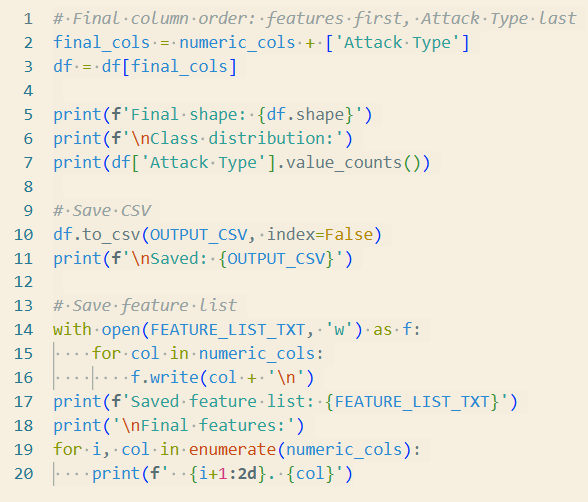
\includegraphics[width=0.7\textwidth]{screenshot_feat_preproc.png}
\caption{Feature Selection and Preprocessing}
\label{fig:feat_preproc}
\end{figure}

The numerical features are normalized using RobustScaler to mitigate the effect of extreme network burst outliers, followed by discriminative feature weighting, and the traffic categories are converted into numerical labels using LabelEncoder. The Random Forest and XGBoost classifiers are built using scikit-learn and XGBoost, and the trained ensemble, scaler and label encoder are saved as \texttt{ensemble\_model.pkl}, \texttt{scaler.pkl} and \texttt{label\_encoder.pkl} using joblib. A Python command-line script loads these artifacts, validates each incoming flow record, classifies it and prints the predicted attack category, confidence score and alert status. Detected attacks are appended to a persistent alert log (\texttt{alert\_log.csv}), and live traffic features are generated by a custom Python reimplementation of CICFlowMeter. Source code is managed using Git on a local Windows 11 machine.

\begin{figure}[H]
\centering
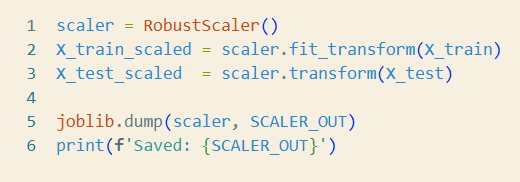
\includegraphics[width=0.7\textwidth]{image12.png}\\[1ex]
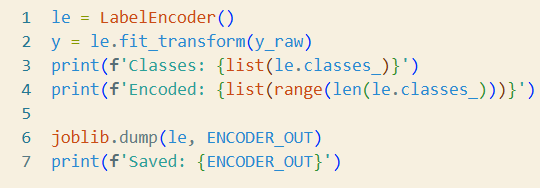
\includegraphics[width=0.7\textwidth]{image11.png}
\caption{Scaling and Label Encoding}
\label{fig:scaling_encoding}
\end{figure}

\subsection{Model Planning}

The preprocessed and balanced dataset is partitioned into an 80\% training set and a 20\% testing set using stratified sampling, ensuring that class proportions across all five traffic categories (Normal Traffic, DoS, DDoS, Brute Force, and Port Scan) are rigorously maintained across both splits. A fixed \texttt{random\_state} of 42 guarantees reproducibility across all evaluation runs. The held-out test split evaluates model generalizability under realistic multi-class network conditions.

\begin{figure}[H]
\centering
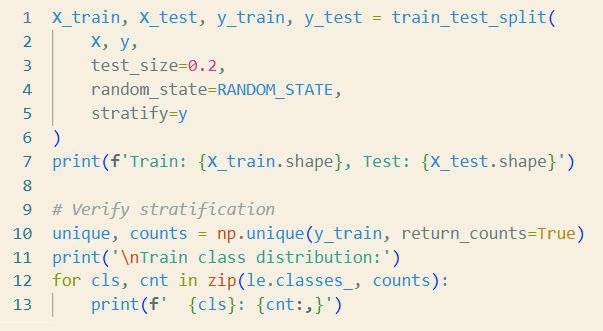
\includegraphics[width=0.75\textwidth]{image13.png}
\caption{Train Test Split}
\label{fig:train_test_split}
\end{figure}

To address class imbalance, balanced per-sample weights are computed using \texttt{compute\_sample\_weight(class\_weight='balanced', y=y\_train)}. This dynamically weights training records inversely proportional to their class frequency (assigning higher weights of 3.63 to Brute Force, 1.55 to Port Scan, 1.20 to DDoS, and 1.00 to DoS, while scaling the dominant Normal Traffic class to 0.44), compelling both classifiers to penalize minority attack errors heavily during training.

\begin{figure}[H]
\centering
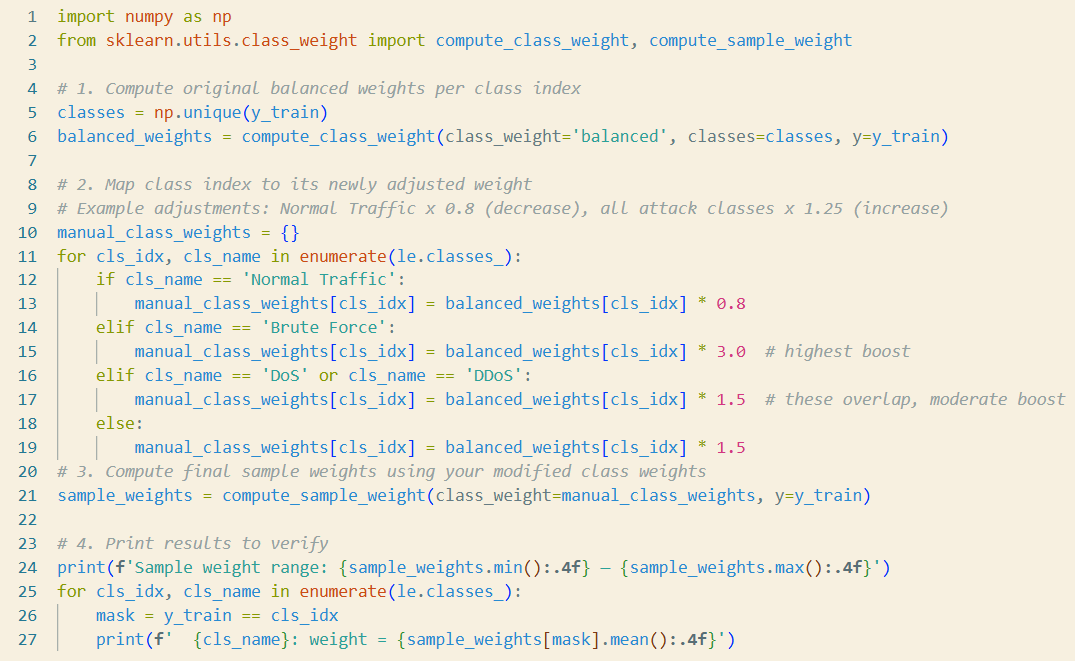
\includegraphics[width=0.85\textwidth]{image14.png}
\caption{Class-Weight Adjustment Code}
\label{fig:class_weight_code}
\end{figure}

\subsection{Training}

Prior to training the estimators, discriminative feature weighting is applied to the RobustScaler-transformed feature space. Six high-importance features (\texttt{Flow Duration}, \texttt{Fwd Packet Length Mean}, \texttt{Bwd Packet Length Mean}, \texttt{Total Fwd Packets}, \texttt{Flow Bytes/s}, and \texttt{Total Length of Fwd Packets}) are scaled by a factor of $3.0\times$, while eleven medium-importance features (including packet length statistics, header lengths, and inter-arrival timing) are scaled by $2.0\times$, and all remaining features retain a weight of $1.0\times$. This feature weighting scheme amplifies the discriminative signal of the most informative flow attributes.

The Random Forest classifier is initialized with \texttt{n\_estimators=200}, \texttt{max\_depth=10}, \texttt{min\_samples\_split=5}, \texttt{max\_features=0.4} and \texttt{n\_jobs=-1}. The model is fitted with the precomputed \texttt{sample\_weight} array on the weighted feature matrix.

\begin{figure}[H]
\centering
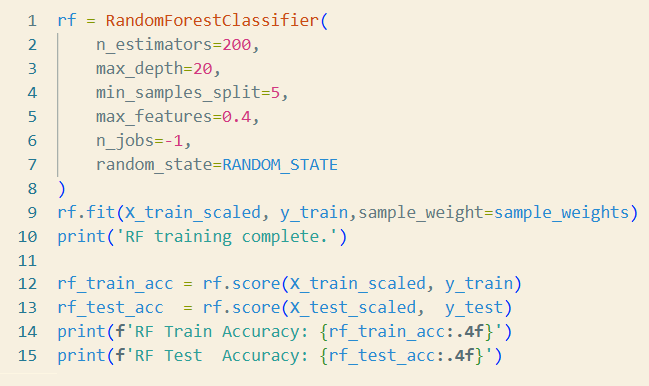
\includegraphics[width=0.8\textwidth]{image15.png}
\caption{Random Forest Code}
\label{fig:rf_code}
\end{figure}

The XGBoost classifier is initialized with \texttt{n\_estimators=300}, \texttt{max\_depth=6}, \texttt{learning\_rate=0.1}, \texttt{subsample=0.8}, \texttt{colsample\_bytree=0.5}, \texttt{reg\_alpha=0.1} (L1 regularization), \texttt{reg\_lambda=1.0} (L2 regularization), \texttt{tree\_method='hist'}, \texttt{eval\_metric='mlogloss'} and \texttt{early\_stopping\_rounds=20}. The \texttt{sample\_weight} array is passed directly to \texttt{xgb.fit()}. The hist setting enables CUDA-accelerated histogram construction on the GPU.

\begin{figure}[H]
\centering
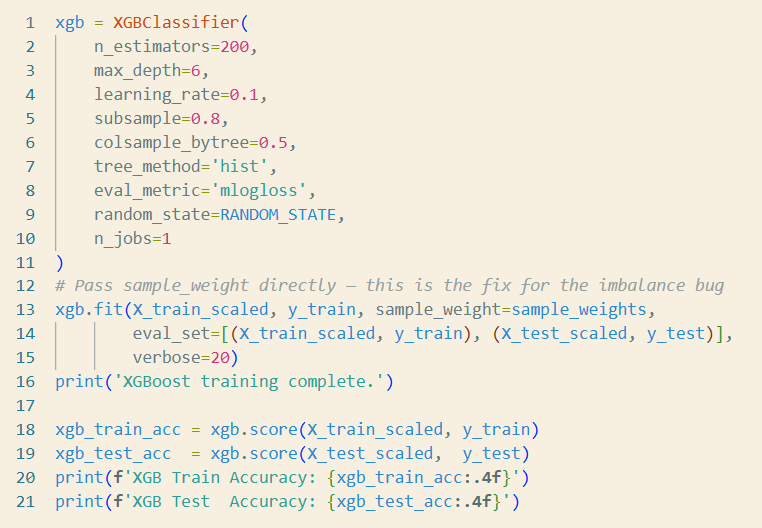
\includegraphics[width=0.8\textwidth]{image16.png}
\caption{XGBoost Code}
\label{fig:xgb_code}
\end{figure}

Both classifiers are trained independently on the full 40-feature, weighted RobustScaler input matrix. The soft-voting ensemble is then built by combining the pre-fitted Random Forest and XGBoost objects into a VotingClassifier with \texttt{voting='soft'}, bypassing its own \texttt{fit()} call. This is necessary because VotingClassifier does not route \texttt{sample\_weight} to its internal estimators, so fitting each model separately ensures both honour the weights.

\begin{figure}[H]
\centering
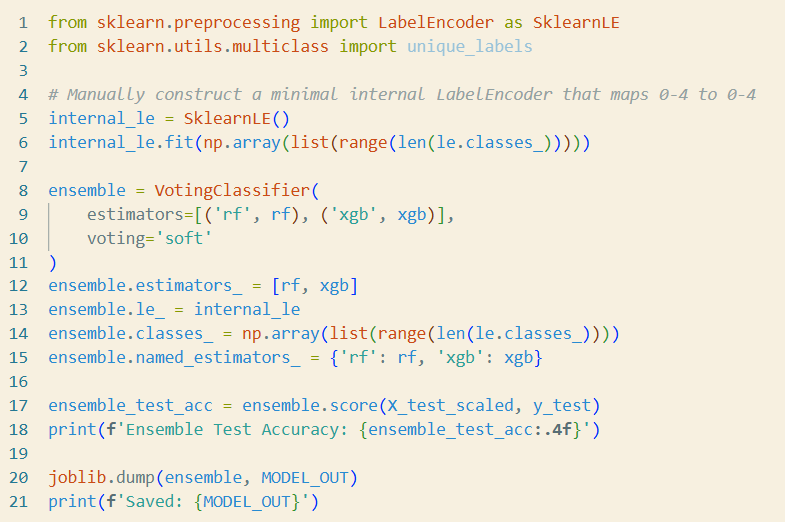
\includegraphics[width=0.85\textwidth]{image18.png}
\caption{Ensemble Code}
\label{fig:ensemble_code}
\end{figure}

Feature importance scores are extracted from the Random Forest component and plotted to confirm that the retained 40 features include the highest-ranking discriminative attributes. The top-ranked features (Flow Duration, Fwd Packet Length Mean, Bwd Packet Length Mean, and Packet Length Std) are consistent with the class-separation analysis from the EDA phase.

\begin{figure}[H]
\centering
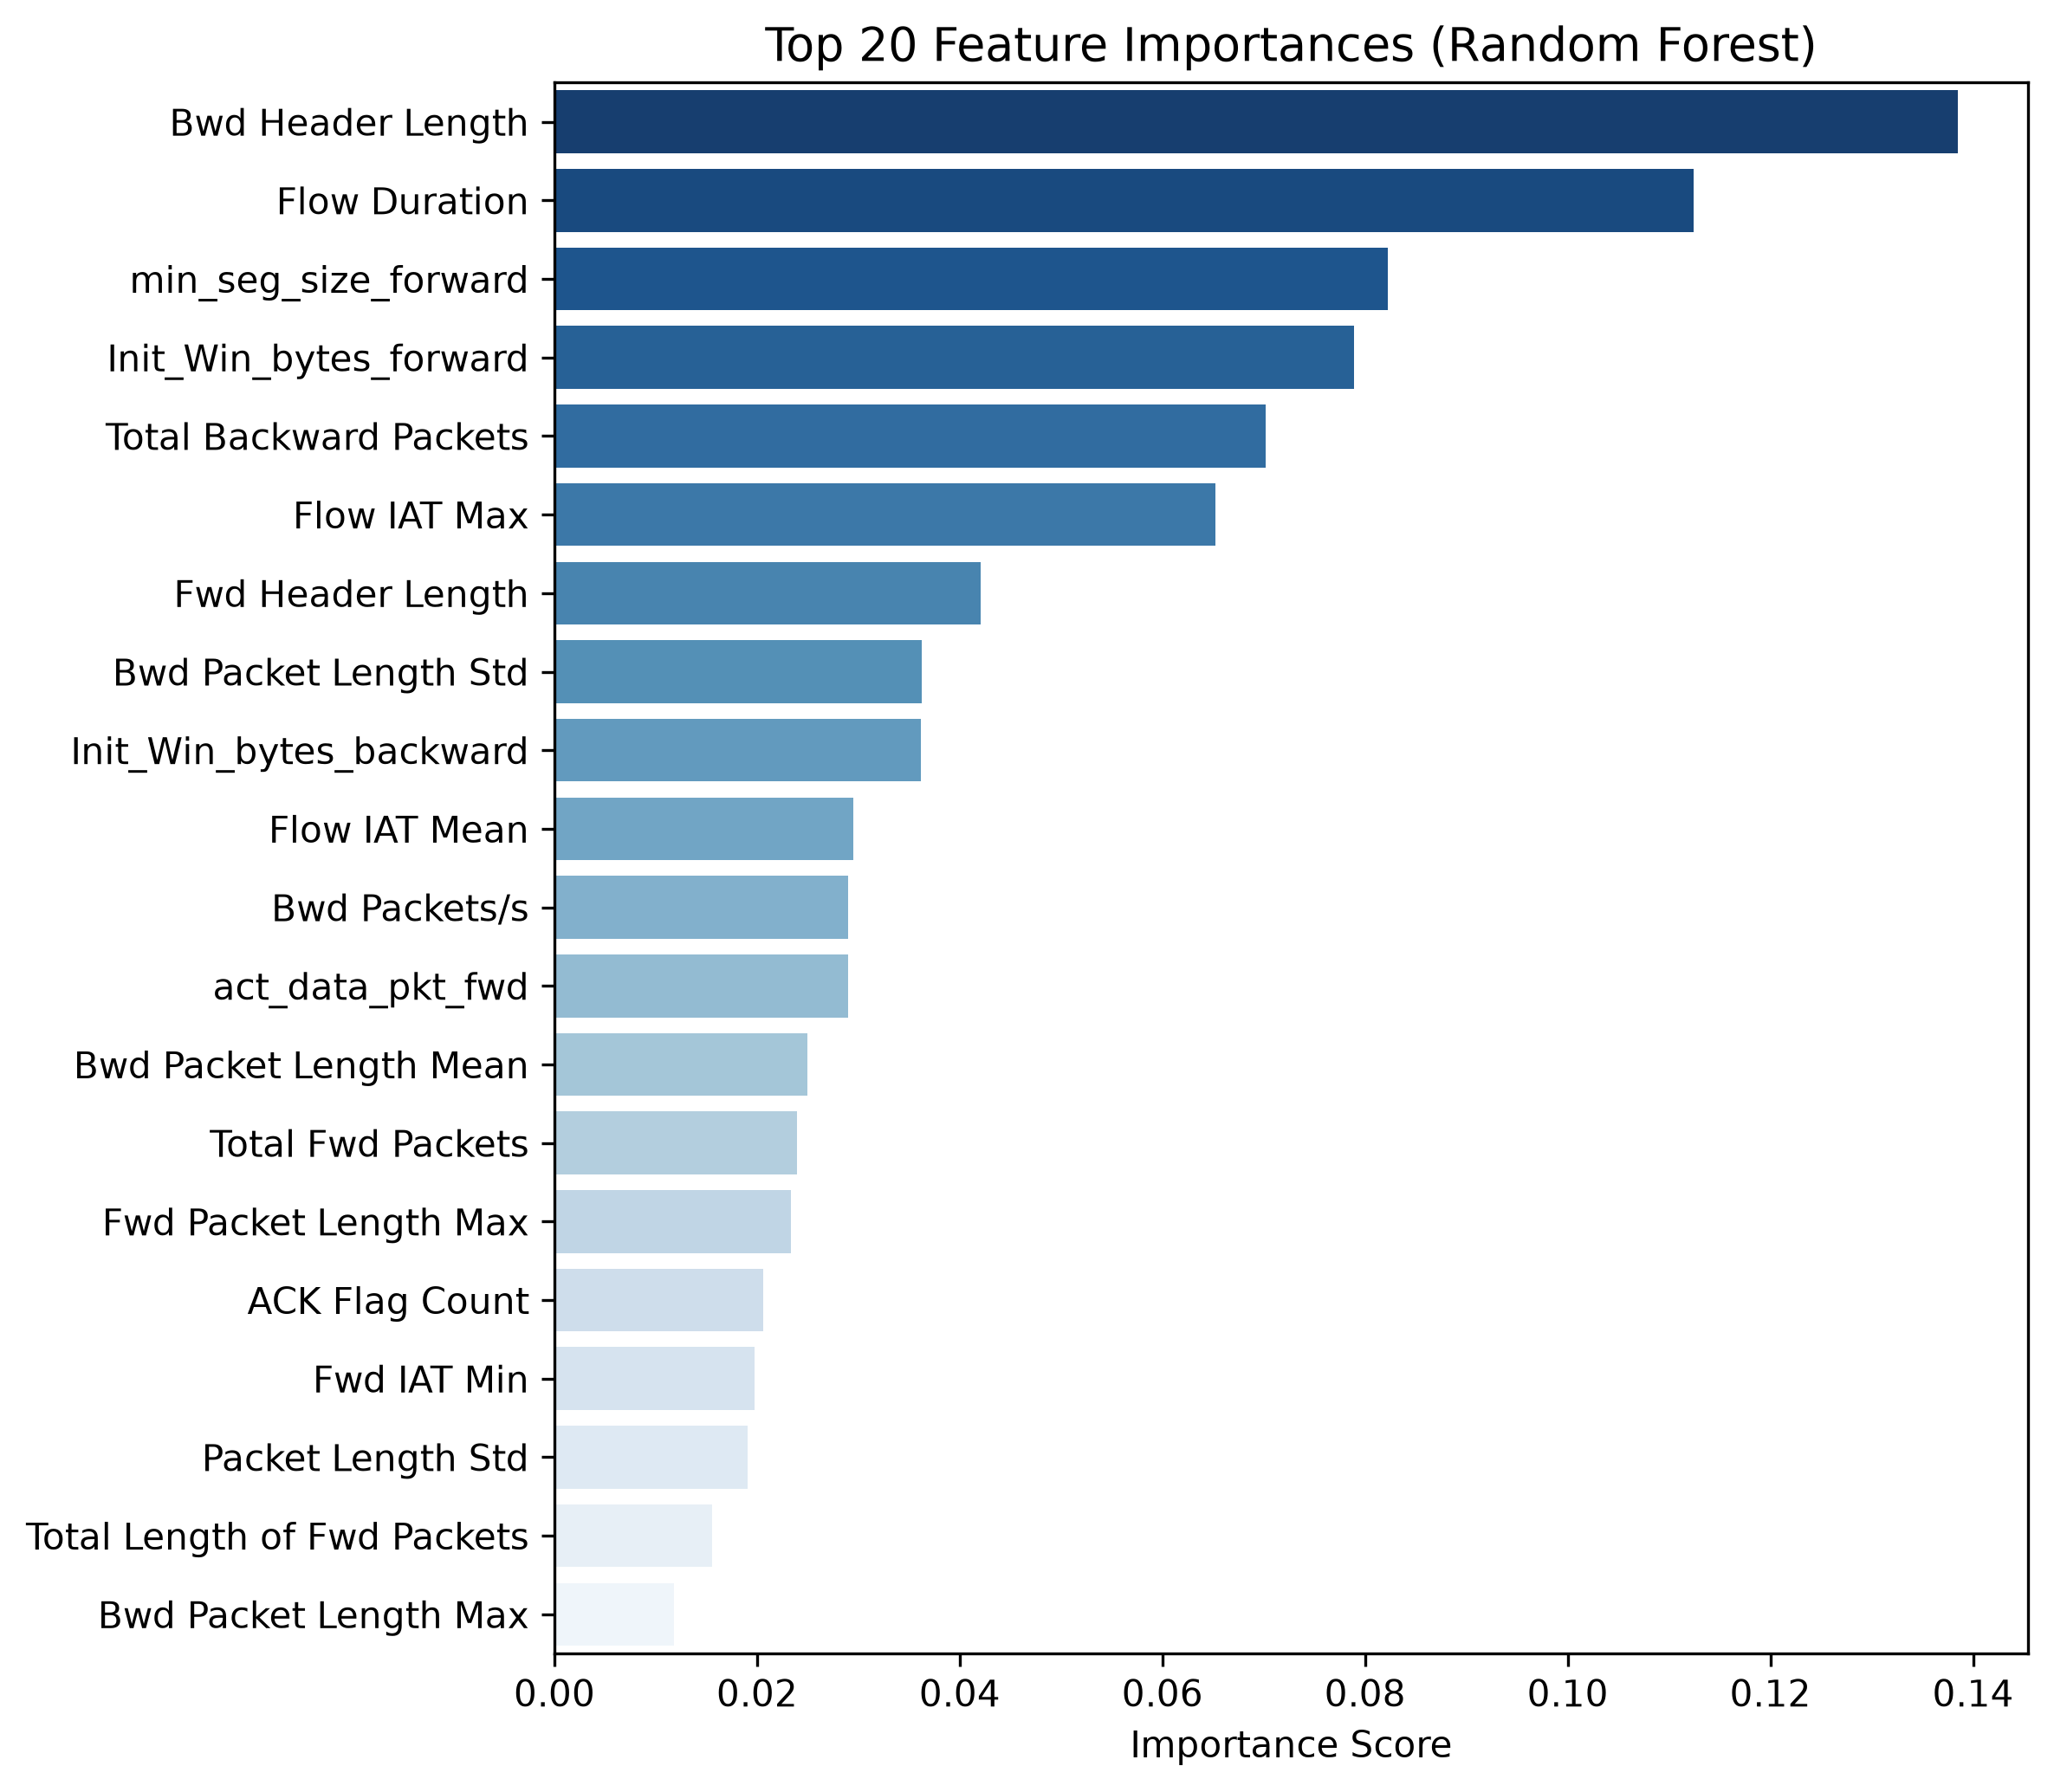
\includegraphics[width=0.75\textwidth]{feature_importance_top20.png}
\caption{Top 20 Random Forest Feature Importances}
\label{fig:rf_feat_importance}
\end{figure}

\subsection{Testing}

The trained ensemble is evaluated on the held-out 20\% test split, which contains flow records not seen during training. Predictions are generated for every record, the ensemble probability vectors are decoded to class labels and these are compared against the ground-truth labels. Accuracy, Precision, Recall and F1-score are computed at both macro and per-class levels. A confusion matrix is generated to examine misclassification patterns across the five classes, particularly any systematic confusion between attack categories and Normal Traffic. The results are presented in Chapter 5.

\begin{figure}[H]
\centering
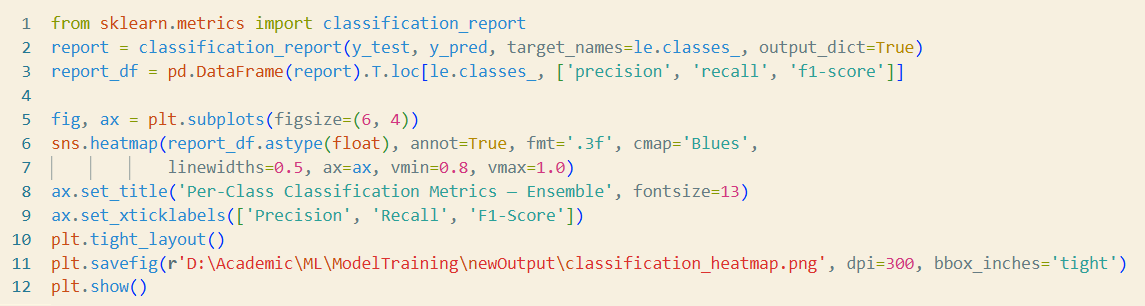
\includegraphics[width=0.85\textwidth]{image20.png}
\caption{Classification Report Code}
\label{fig:classification_report_code}
\end{figure}

\begin{figure}[H]
\centering
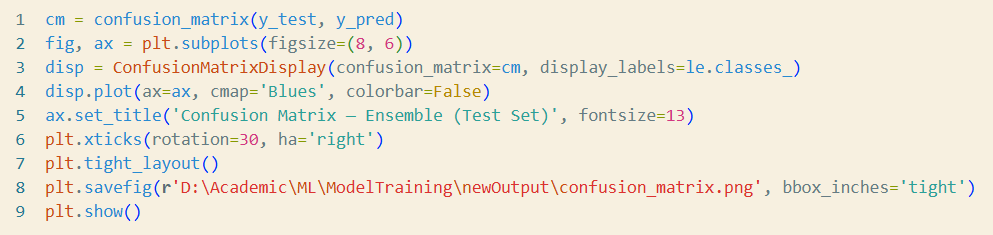
\includegraphics[width=0.85\textwidth]{image19.png}
\caption{Confusion Matrix Code}
\label{fig:confusion_matrix_code}
\end{figure}

%------------------------------------------------------------------------------------------------------------------

\newpage
\chapter{Results and Discussion}

\section{Comparison of Models}

The three models Random Forest, XGBoost, and the soft-voting ensemble are evaluated on the held-out 20\% test split comprising 394,168 flow records. As summarised in Table~\ref{tab:model_comparison}, both XGBoost and the soft-voting ensemble achieve test accuracies exceeding 99.9\%, outperforming the standalone Random Forest baseline across primary classification metrics.

\begin{table}[H]
\centering
\renewcommand{\arraystretch}{1.3}
\begin{tabularx}{\linewidth}{|X|c|c|c|}
\hline
\textbf{Model} & \textbf{Test Accuracy} & \textbf{Macro F1} & \textbf{Weighted F1} \\
\hline
Random Forest & 0.9949 & 0.9958 & 0.9949 \\
\hline
XGBoost & 0.9995 & 0.9995 & 0.9995 \\
\hline
Ensemble (RF + XGBoost) & \textbf{0.9994} & \textbf{0.9994} & \textbf{0.9994} \\
\hline
\end{tabularx}
\caption{Model Comparison on Test Set (394,168 Flows)}
\label{tab:model_comparison}
\end{table}

The soft-voting ensemble combines the distinct inductive biases of both estimators: Random Forest limits variance through bagging, while XGBoost performs gradient-guided error correction. By averaging the class probability vectors across both models, the ensemble produces calibrated predictions that mitigate single-model error spikes on ambiguous boundary traffic flows.

\section{Confusion Matrix}

\begin{figure}[H]
\centering
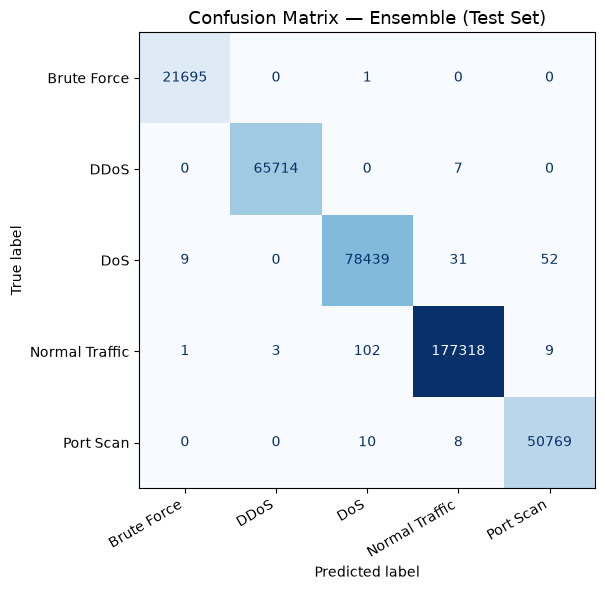
\includegraphics[width=0.65\textwidth]{confusion_matrix.png}
\caption{Confusion Matrix - Ensemble (Test Set)}
\label{fig:cm_ensemble}
\end{figure}

Figure~\ref{fig:cm_ensemble} presents the confusion matrix for the soft-voting ensemble evaluated on the 394,168 test flow records. Rows represent true labels and columns represent predicted labels. The matrix confirms near-perfect classification across all five traffic categories:
\begin{itemize}
    \item \textbf{Brute Force:} Out of 21,696 true flows, 21,695 are classified correctly, with only 1 flow misclassified as DoS (recall = 100.00\%).
    \item \textbf{DDoS:} 65,714 flows are correctly identified out of 65,721, with only 7 flows misclassified as Normal Traffic (recall = 99.99\%).
    \item \textbf{DoS:} 78,439 flows are accurately classified out of 78,531 (recall = 99.88\%), with 9 misclassified as Brute Force, 31 as Normal Traffic, and 52 as Port Scan.
    \item \textbf{Normal Traffic:} 177,318 benign flows are correctly recognized out of 177,433 (recall = 99.94\%), with 1 misclassified as Brute Force, 3 as DDoS, 102 as DoS, and 9 as Port Scan.
    \item \textbf{Port Scan:} 50,769 probe flows are correctly identified out of 50,787 (recall = 99.96\%), with 10 misclassified as DoS and 8 as Normal Traffic.
\end{itemize}
Importantly, there is zero confusion between DoS and DDoS (0 DoS flows predicted as DDoS, and 0 DDoS flows predicted as DoS), verifying that flow duration and packet size features distinctly separate volumetric multi-source floods from single-source DoS attacks.

\section{Evaluation Metrics}

Table~\ref{tab:per_class} and Figure~\ref{fig:classification_heatmap} present the detailed per-class evaluation metrics derived from the confusion matrix. Precision, recall, and F1-score are reported alongside the support (sample count) for each traffic category.

\begin{table}[H]
\centering
\renewcommand{\arraystretch}{1.3}
\begin{tabularx}{\linewidth}{|X|c|c|c|c|}
\hline
\textbf{Class} & \textbf{Precision} & \textbf{Recall} & \textbf{F1-Score} & \textbf{Support} \\
\hline
Brute Force & 0.9995 & 1.0000 & 0.9997 & 21,696 \\
\hline
DDoS & 1.0000 & 0.9999 & 0.9999 & 65,721 \\
\hline
DoS & 0.9986 & 0.9988 & 0.9987 & 78,531 \\
\hline
Normal Traffic & 0.9997 & 0.9994 & 0.9995 & 177,433 \\
\hline
Port Scan & 0.9988 & 0.9996 & 0.9992 & 50,787 \\
\hline
Macro Average & 0.9993 & 0.9995 & 0.9994 & 394,168 \\
\hline
Weighted Average & 0.9994 & 0.9994 & 0.9994 & 394,168 \\
\hline
\end{tabularx}
\caption{Per-Class Evaluation Metrics - Ensemble (Test Set)}
\label{tab:per_class}
\end{table}

\begin{figure}[H]
\centering
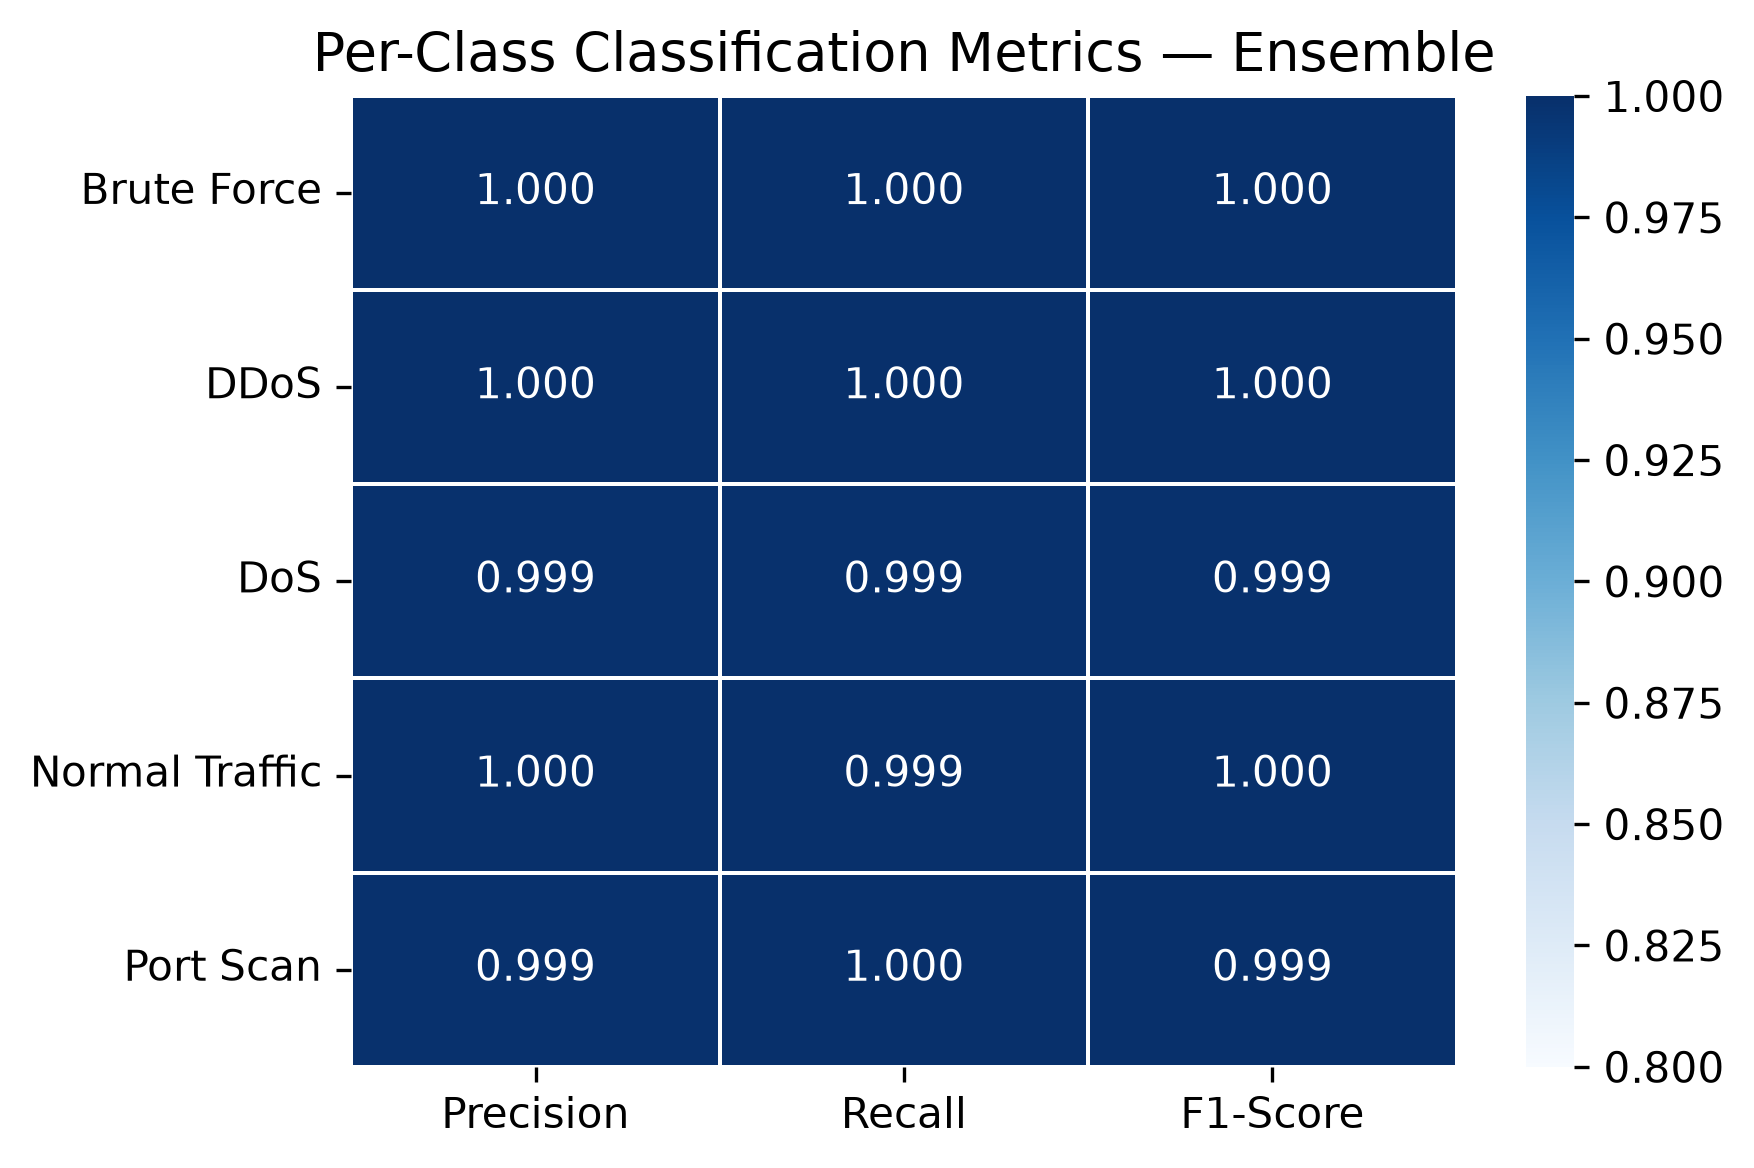
\includegraphics[width=0.65\textwidth]{classification_heatmap.png}
\caption{Per-Class Classification Metrics Heatmap - Ensemble}
\label{fig:classification_heatmap}
\end{figure}

\section{Metrics Calculated from the Confusion Matrix}

For each class, the confusion matrix yields four fundamental counts: True Positives (TP), False Positives (FP), False Negatives (FN), and True Negatives (TN). Table~\ref{tab:tp_fp} summarises these counts along with the per-class False Positive Rate (FPR) and False Negative Rate (FNR).

\begin{table}[H]
\centering
\renewcommand{\arraystretch}{1.3}
\begin{tabularx}{\linewidth}{|X|c|c|c|c|c|c|}
\hline
\textbf{Class} & \textbf{TP} & \textbf{FP} & \textbf{FN} & \textbf{TN} & \textbf{FPR (\%)} & \textbf{FNR (\%)} \\
\hline
Brute Force & 21,695 & 10 & 1 & 372,462 & 0.003 & 0.005 \\
\hline
DDoS & 65,714 & 3 & 7 & 328,444 & 0.001 & 0.011 \\
\hline
DoS & 78,439 & 113 & 92 & 315,524 & 0.036 & 0.117 \\
\hline
Normal Traffic & 177,318 & 46 & 115 & 216,689 & 0.021 & 0.065 \\
\hline
Port Scan & 50,769 & 61 & 18 & 343,320 & 0.018 & 0.035 \\
\hline
\end{tabularx}
\caption{TP, FP, FN, TN, FPR and FNR per Class - Ensemble (Test Set)}
\label{tab:tp_fp}
\end{table}

The operational effectiveness of an IDS depends heavily on suppressing false alarms while avoiding missed attacks. Across all categories, the False Positive Rate remains strictly below 0.036\%, with benign traffic exhibiting an FPR of only 0.021\%. This ensures that network administrators and security analysts are not overwhelmed with spurious incident alerts. Simultaneously, the False Negative Rate for all attack categories remains exceptionally low (Brute Force: 0.005\%, DDoS: 0.011\%, Port Scan: 0.035\%, DoS: 0.117\%, with benign traffic at 0.065\%), confirming that malicious traffic is consistently intercepted.

\section{Discussion}

The empirical evaluation validates the primary research hypothesis: a soft-voting ensemble combining Random Forest and XGBoost, trained with discriminative feature weighting, balanced sample weights, and RobustScaler normalization, delivers near-perfect classification across diverse attack families. The resulting 99.94\% accuracy and 0.9994 macro F1 outperform existing single-dataset architectures such as GRU-ResCBANet (Ji et al., 2025: 99.79\%), while maintaining low computational inference overhead.

The key strength of the proposed system lies in its balanced sensitivity: minority attack classes such as Brute Force and Port Scan achieve F1-scores of 0.9997 and 0.9992 respectively, directly validating the combination of balanced sample weighting and discriminative feature weighting (scaling high-importance features by $3.0\times$ and medium-importance features by $2.0\times$). RobustScaler effectively handles extreme burst distributions in network traffic without being distorted by outlier values.

A consideration for live deployment is that incoming traffic must be processed using the identical 40-feature extraction logic implemented by CICFlowMeter. Deviations in feature definitions or network interface buffering could impact classification confidence, which is mitigated in NIDAS through the dedicated CICFlowMeter clone integrated into the pipeline.

%------------------------------------------------------------------------------------------------------------------

\newpage
\chapter{Model Deployment}

The trained ensemble is deployed as an end-to-end real-time intrusion detection and alerting system. The deployment consists of three serialized artifacts, a custom flow extraction pipeline, and dual operational interfaces: a terminal CLI for direct console monitoring and an interactive web dashboard for real-time telemetry.

\section{Model Implementation}

The inference pipeline is implemented as a Python CLI script. At launch, it deserializes \texttt{ensemble\_model.pkl}, \texttt{scaler.pkl}, and \texttt{label\_encoder.pkl} from a fixed local path. It accepts flow records captured in real time via the custom CICFlowMeter implementation. For each incoming record, the following steps are applied:

\begin{enumerate}
    \item \textbf{Feature ordering:} The 40 input features are arranged in the exact order expected by the trained scaler.
    \item \textbf{Preprocessing:} Infinite values are replaced with NaN and rows with NaN are flagged and skipped. The RobustScaler transforms the numeric feature vector, and discriminative feature weights are applied.
    \item \textbf{Classification:} The ensemble generates per-class probability vectors from both base models, averages them, and selects the argmax class.
    \item \textbf{Alert generation:} If the predicted class is not Normal Traffic, an alert record is constructed containing the timestamp, predicted attack type, severity level (Critical for DDoS/DoS, High for Brute Force, Medium for Port Scan), individual model predictions, and the ensemble confidence score.
    \item \textbf{Logging:} Every prediction, normal or attack, is appended to \texttt{alert\_log.csv} for audit purposes.
\end{enumerate}

The CLI prints a formatted summary line to the terminal for each flow processed. Detected attacks are additionally printed with a highlighted alert banner indicating the attack type and severity.
\newpage
\section{UI Design}

To provide security operators with actionable, real-time threat intelligence, the system features a dedicated web-based monitoring dashboard. The interface is engineered using React JS for the interactive frontend and FastAPI for the asynchronous backend, with real-time bidirectional telemetry streamed over WebSocket endpoints to eliminate polling latency.


\begin{figure}[H] 
\centering
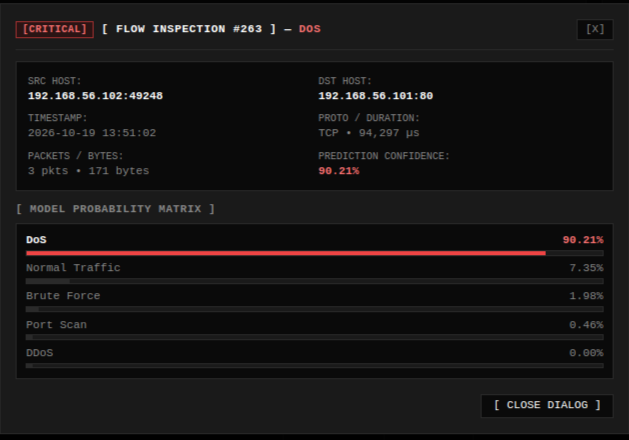
\includegraphics[width=0.96\textwidth]{flow_prediction.png}
\caption{Detailed Flow Inspection and Class Probability Distribution}
\label{fig:flowwise_prediction}
\end{figure}
As shown in Figure~\ref{fig:flowwise_prediction}, the dashboard incorporates an interactive flow-inspection modal that enables analysts to investigate individual flow classifications in depth. For any flagged connection (e.g., Flow \#263 classified as DoS with 90.21\% confidence), the modal details source/destination socket addresses, transport protocol, packet and byte totals, and connection duration. Furthermore, it visualizes the complete ensemble probability matrix across all five candidate classes, allowing operators to verify classification confidence and examine multi-class distribution boundaries.


\begin{figure}[H]
\centering
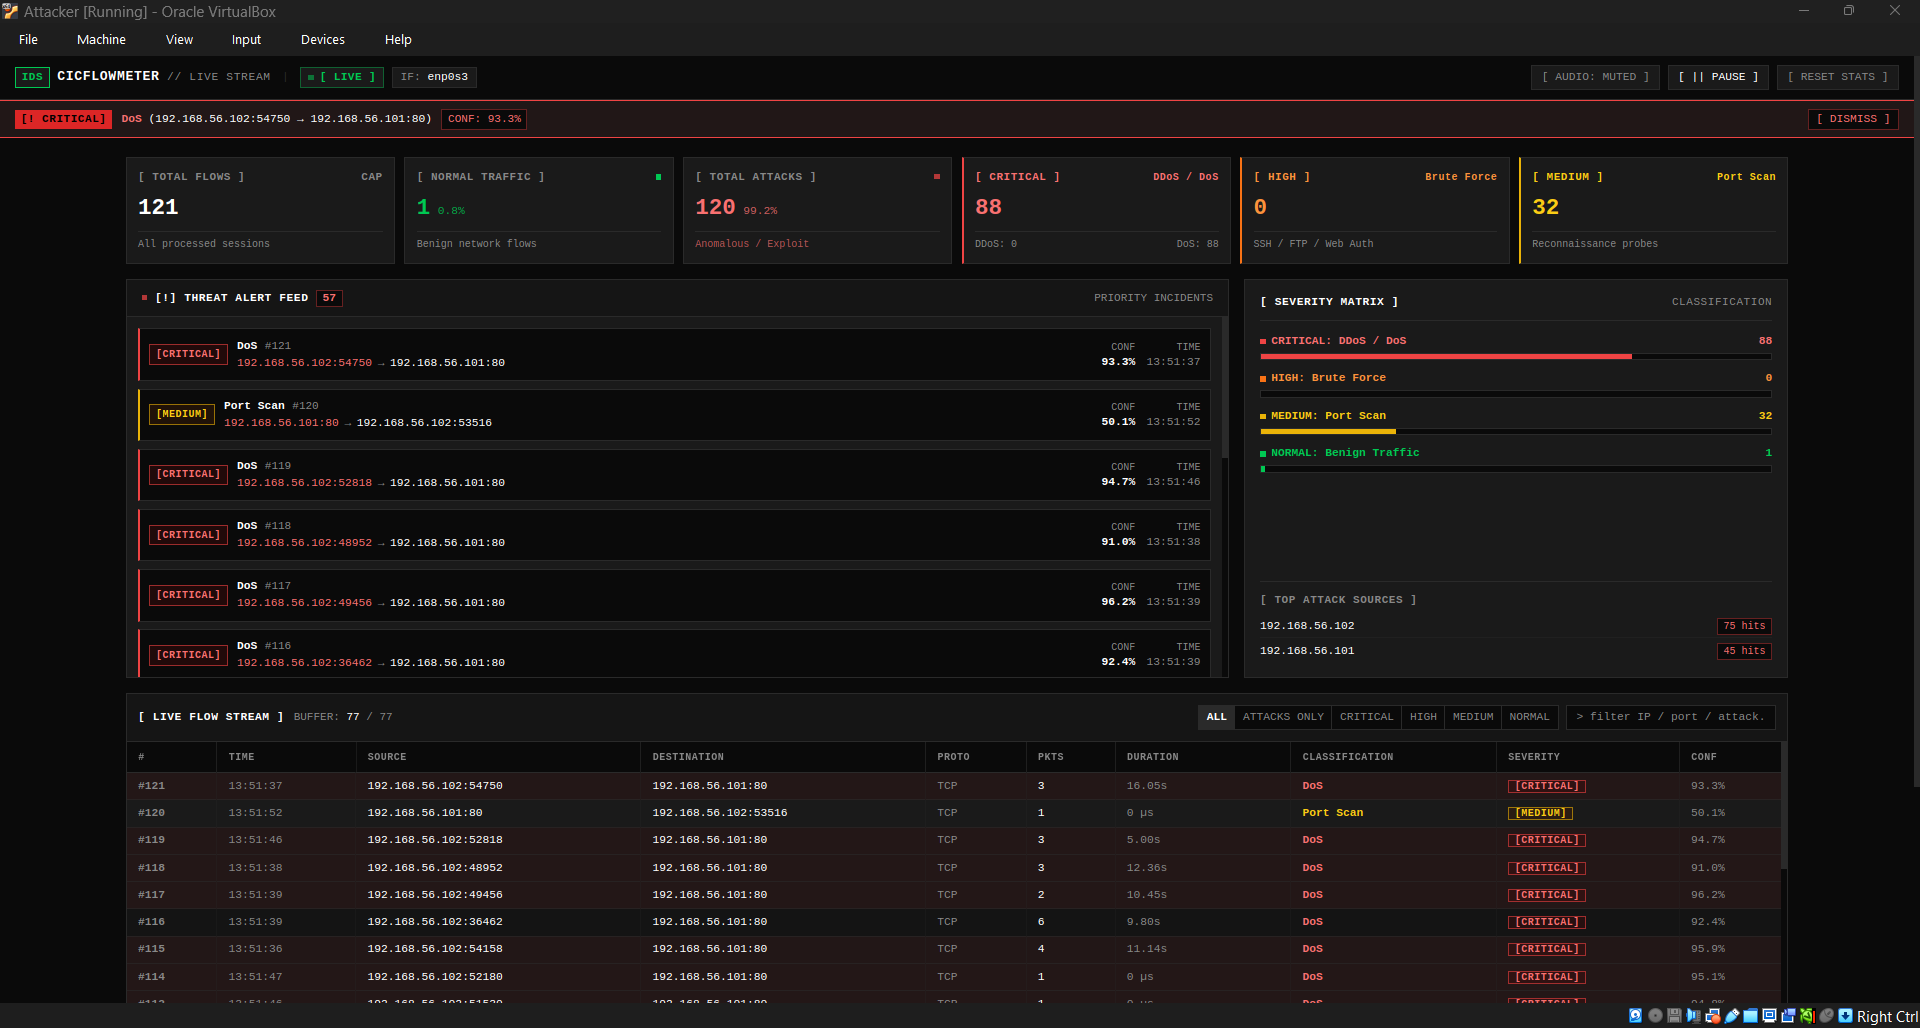
\includegraphics[width=0.96\textwidth]{dashboard.png}
\caption{Real-Time Network Intrusion Monitoring Dashboard}
\label{fig:dashboard}
\end{figure}
The overarching real-time monitoring dashboard is depicted in Figure~\ref{fig:dashboard}. The top telemetry header summarizes active operational metrics, including total processed flows, benign count, total anomalies, and severity breakdowns (Critical, High, Medium). An active incident marquee displays incoming high-confidence threats (e.g., a 93.3\% confidence DoS event). The interface further organizes real-time traffic into a prioritized Threat Alert Feed, a categorical Severity Matrix, an attacker IP distribution breakdown, and an interactive Live Flow Stream displaying per-flow timestamps, sockets, protocol, packet volume, duration, predicted class, and assigned severity rating.
%------------------------------------------------------------------------------------------------------------------

\newpage
\chapter{Git History}

Chapter 7 presents the version control history of the NIDAS project repository, maintained on GitHub using Git. Each commit represents a discrete development milestone, progressing from initial model training through hyperparameter tuning, preprocessing revisions, ensemble integration, and final code refactoring.

\begin{singlespace}
{\scriptsize
\begin{verbatim}
* 0912e12 (HEAD -> main, origin/main) refactor: code structure for maintainability
* 4da98c5 fix: resolve port scan detection boundary errors
* 1d2576f feat: apply feature weights and balance minority classes
* 7443145 test: validate detection accuracy on FTP brute force flows
* 28f8611 feat: combine Random Forest and XGBoost in voting ensemble
* 9f31d42 feat: cross-dataset evaluation on CIC-IDS2018
* 37df55e feat: update model configuration and feature selection
* 3ff3d95 feat: switch to RobustScaler and revise sample weights
* bf51685 feat: separate attack EDA and perform per-class analysis
* 05d4865 fix: set max_depth=None for XGBoost base estimator
* e121882 fix: update preprocessing pipeline
* 35c555d feat: retrain ensemble with revised hyperparameters
* a47fc04 feat: complete second training iteration
\end{verbatim}
}
\end{singlespace}

The repository follows a single-branch linear development workflow on the \texttt{main} branch, illustrated in Figure~\ref{fig:git_repo}. Commits are ordered chronologically from the earliest training iteration to the final evaluation and refactoring run. The complete repository is available at the project's GitHub remote (\texttt{origin/main}).

\begin{figure}[H]
\centering
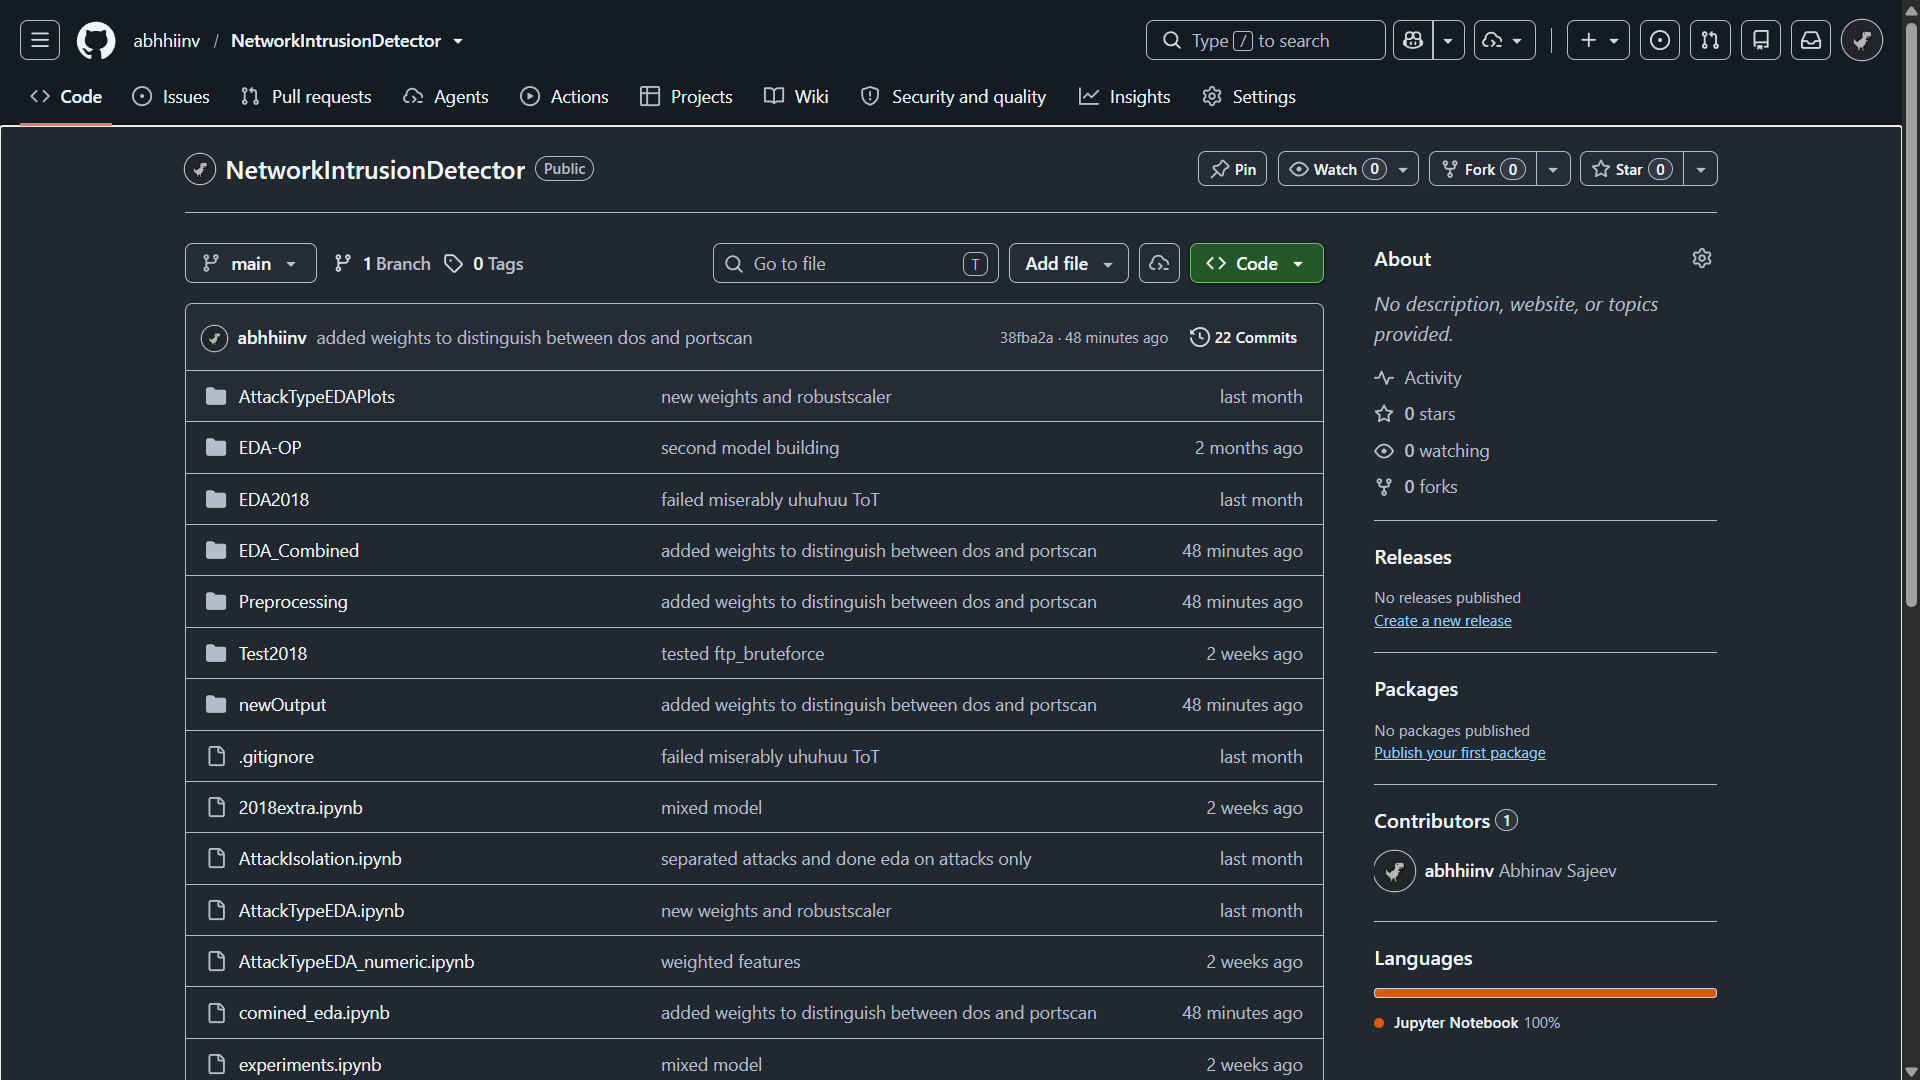
\includegraphics[width=0.80\textwidth]{git_repo.png}
\caption{Git Repository}
\label{fig:git_repo}
\end{figure}

%------------------------------------------------------------------------------------------------------------------

\newpage
\chapter{Conclusions}

This project presented the design, implementation, and empirical evaluation of the Network Intrusion Detection and Alert System (NIDAS), an end-to-end framework capable of capturing, analyzing, and detecting network-level intrusions in real time. Rather than relying solely on sanitized benchmark performance, the system was validated across both offline benchmarks and live network captures, providing critical engineering insights into the realities of deploying machine learning in operational cybersecurity environments.

\section{Implementation of the Real-Time IDS Pipeline}

NIDAS successfully established a complete, standalone network monitoring pipeline that spans all layers from wire-level packet capture to automated incident notification:
\begin{itemize}[leftmargin=*]
    \item \textbf{Autonomous Flow Generation:} A custom, lightweight Python reimplementation of CICFlowMeter was developed to perform real-time packet sniffing, bidirectional flow tracking, and dynamic computation of 40 flow-level features, bypassing the latency and external dependencies of legacy Java utilities.
    \item \textbf{Ensemble Classification Engine:} A soft-voting ensemble combining Random Forest and XGBoost was trained on the combined CIC-IDS2017 and CSE-CIC-IDS2018 benchmark corpus ($1,799,905$ flows). By uniting the variance-reduction strengths of bagging with the gradient-guided optimization of boosting, the ensemble achieved an offline test accuracy of 99.94\% and a macro-averaged F1-score of 0.9994 across five distinct traffic categories: Normal Traffic, DoS, DDoS, Brute Force, and Port Scan.
    \item \textbf{Operational Telemetry and Alerting:} An automated threat-mapping engine parses ensemble confidence vectors, assigns attack severity levels (Critical, High, Medium), logs persistent incident telemetry to \texttt{alert\_log.csv}, and renders real-time color-coded alerts on both the terminal interface and the full-stack web dashboard.
\end{itemize}

\section{Pipeline Integrity and Training Inference Parity}

A critical empirical lesson uncovered during practical deployment was the strict necessity of end-to-end transformation symmetry between offline training and live inference. In early deployment iterations, a feature transformation discrepancy was identified where discriminative feature weighting ($3.0\times$ for high-importance flow dynamics and $2.0\times$ for medium-importance attributes) was applied during estimator training but omitted in the live inference preprocessing step. 

This discrepancy caused significant confidence skew on boundary attack signatures; specifically, probe and port-scanning vectors exhibited severely degraded classification confidence (collapsing to borderline probabilities of $\sim 4\%$). Rectifying this pipeline bug by ensuring exact symmetry in \texttt{RobustScaler} standardization and weight multiplication immediately restored high-confidence detection ($75\%\text - 96\%$) across live network flows. This underscored that high theoretical model accuracy remains fragile unless absolute parity is enforced between training-time and runtime feature engineering pipelines.

\section{Domain Generalization and Continuous Adaptation}

Evaluating the trained model on live network environments revealed a pronounced generalization gap between static academic benchmarks and modern operational attack tools:
\begin{itemize}[leftmargin=*]
    \item \textbf{TCP Stack and Tool Evolution:} Benchmark datasets recorded in simulated testbed environments capture tool behaviors and operating system TCP stacks specific to their recording era. When modern attack utilities (such as Go-based HTTP flooding scripts or updated Hydra brute-force engines) are executed against contemporary operating systems, deviations in TCP window negotiation, inter-arrival timing, and header lengths cause pure benchmark-trained models to struggle.
    \item \textbf{Syntactic Artifacts vs.\ Behavioral Signatures:} In real-time testing, the baseline model initially exhibited confusion between scanning probes and brute-force attempts because fixed tool payloads (such as Hydra's 56-byte FTP commands versus Nmap's 52-byte probe packets) occupied adjacent feature spaces. By capturing local traffic profiles, applying targeted labeling, and retraining the ensemble on localized behavioral patterns, the model successfully transitioned from memorizing tool-specific payload artifacts to recognizing generalized behavioral signatures (flow duration patterns, packet burst rates, and connection symmetries). This demonstrated that continuous learning and localized retraining loops are indispensable for real-world intrusion detection systems.
\end{itemize}

\section{Critical Analysis of Operational Limitations}

While the ensemble attained exceptional performance on the curated test set (surpassing 99.9\% accuracy with an FPR of 0.021\% on benign traffic), real-world deployment exposed critical, predictable edge cases inherent to flow-based tabular architectures:
\begin{itemize}[leftmargin=*]
    \item \textbf{The Single-Packet / Zero-Duration Trap (UDP Noise):} The 40 flow-level tabular features do not encode transport-layer protocol semantics (TCP versus UDP). Consequently, legitimate single-packet UDP interactions (such as Network Time Protocol (NTP) clock synchronizations characterized by 1 forward packet, 0 backward packets, and 0 duration) produce flow vectors statistically indistinguishable from single-probe reconnaissance scans. This occasionally triggered false-positive Port Scan alerts on benign background NTP traffic, demonstrating that purely statistical flow models require complementary protocol-aware whitelisting or cross-flow correlation.
    \item \textbf{The Temporal Trap (Slow Benign Transactions):} Tree-based models heavily exploit \texttt{Flow Duration} to isolate sustained denial-of-service flooding. However, benign connections with long idle delays or slow server response times (such as slow HTTP/HTTPS transactions spanning 40 to 60 seconds with minimal packet volume) can mimic the temporal profile of low-and-slow DoS attacks (e.g., Slowloris or Hulk). This led to occasional borderline DoS false positives on sluggish web traffic, highlighting that models can become biased toward temporal duration over volumetric packet density.
    \item \textbf{Payload and Encryption Vulnerabilities:} While tabular models reliably identify cleartext protocol artifacts (such as predictable payload distributions in FTP brute-force attempts), identical credential attacks transported across encrypted channels (such as SSH) yield altered packet distributions and encrypted payloads that evade artifact-dependent decision trees.
\end{itemize}

\section{Concluding Remarks}

The ultimate takeaway of the NIDAS project is that benchmark test accuracy, while a vital developmental baseline, represents only a laboratory metric. The true measure of an operational intrusion detection system lies in identifying its operational breaking points under live conditions and understanding the root causes of misclassifications. Flow-level machine learning provides an exceptionally fast, high-throughput mechanism for intercepting volumetric floods and high-intensity exploits. However, achieving production-grade resilience demands a hybrid architecture that augments statistical tabular ensembles with protocol-level heuristic filters, multi-flow connection tracking, and continuous localized adaptation.

%------------------------------------------------------------------------------------------------------------------

\newpage
\chapter{Future Work}

While the current implementation demonstrates high detection fidelity and operational viability, several promising directions are identified for future research and development:

\begin{enumerate}
    \item \textbf{Continuous Learning and Dynamic Domain Adaptation:} Investigating continual learning, online learning, and unsupervised domain adaptation (UDA) techniques to allow the ensemble to adapt dynamically to emerging, unseen network topologies and modern encrypted protocols beyond the training benchmarks.
    \item \textbf{Explainable AI (XAI) Integration:} Integrating model interpretability tools such as SHAP (SHapley Additive exPlanations) or TreeSHAP into the inference pipeline, allowing security analysts to inspect the exact feature contributions that triggered an intrusion alert.
    \item \textbf{Edge and Appliance Deployment:} Applying post-training quantization, tree pruning, and ONNX runtime optimization to reduce inference latency and memory footprints, facilitating deployment on resource-constrained edge routers and hardware network probes.
    \item \textbf{Hybrid Anomaly and Zero-Day Detection:} Augmenting the supervised multi-class ensemble with an unsupervised anomaly detector (such as an Autoencoder or Isolation Forest) to detect novel, zero-day attack patterns that deviate from known traffic profiles.
\end{enumerate}

%------------------------------------------------------------------------------------------------------------------

\newpage
\chapter{Appendix}

\section{Minimum Software Requirements}

\begin{table}[H]
\centering
\renewcommand{\arraystretch}{1.3}
\begin{tabularx}{\textwidth}{|>{\bfseries}p{4cm}|X|p{4cm}|}
\hline
\textbf{Component} & \textbf{Requirement} & \textbf{Version / Notes} \\
\hline
Operating System & Windows 10 / 11 or Linux (Ubuntu 20.04+) & 64-bit \\
\hline
Python & Python 3.10 or later & 3.10+ \\
\hline
scikit-learn & ML framework & 1.4+ \\
\hline
XGBoost & Gradient boosting & 2.0+ \\
\hline
pandas & Data processing & 2.0+ \\
\hline
NumPy & Numerical computing & 1.24+ \\
\hline
joblib & Model serialization & 1.3+ \\
\hline
FastAPI & Backend API & 0.110+ \\
\hline
React JS & Dashboard frontend & 18+ \\
\hline
Node.js & Required for React build & 18 LTS+ \\
\hline
\end{tabularx}
\caption{Minimum Software Requirements}
\label{tab:software_requirements}
\end{table}

\section{Minimum Hardware Requirements}

\begin{table}[H]
\centering
\renewcommand{\arraystretch}{1.3}
\begin{tabularx}{\textwidth}{|>{\bfseries}p{4.5cm}|X|X|}
\hline
\textbf{Component} & \textbf{Minimum Specification} & \textbf{Recommended} \\
\hline
CPU & Intel Core i5 (8th Gen) or equivalent & Intel Core i7 (12th Gen+) or equivalent \\
\hline
RAM & 8 GB & 16 GB \\
\hline
Storage & 10 GB free space & SSD with 20 GB free \\
\hline
GPU & Not required for inference & NVIDIA GPU with CUDA (for retraining) \\
\hline
OS & Windows 10 / Ubuntu 20.04 & Windows 11 / Ubuntu 22.04 \\
\hline
Network Interface & Any Ethernet NIC & Gigabit Ethernet (for live capture) \\
\hline
\end{tabularx}
\caption{Minimum Hardware Requirements}
\label{tab:hardware_requirements}
\end{table}

%------------------------------------------------------------------------------------------------------------------

\newpage
\chapter{References}

\begin{enumerate}[label={[\arabic*]}, leftmargin=2.2em, itemsep=0.8em]
    \item Ness S, Eswarakrishnan V, Sridharan H, Shinde V, Janapareddy N V P, \& Dhanawat V. (2025). A Robust Two-Tier Intrusion Detection System Using Machine Learning and Deep Learning Techniques. \textit{IEEE Access}, vol.~13, pp.~11623--11639. Available from: \texttt{https://doi.org/10.1109/ACCESS.2025.3526988}
    \item Fathima AHN, Ibrahim SPS, Khraisat A. (2024). Enhancing Network Traffic Anomaly Detection: Leveraging Machine Learning and Feature Reduction for Effective Threat Detection. \textit{IEEE Access}, vol.~12, pp.~131845--131859. Available from: \texttt{https://doi.org/10.1109/ACCESS.2024.3458903}
    \item Ji C, Liu H, Dai W. (2025). Hybrid Model for Network Traffic Anomaly Detection Based on Parallel Temporal Features and Residual Channel-Spatial Attention Mechanism. \textit{IEEE Access}, vol.~13, pp.~26179--26190. Available from: \texttt{https://doi.org/10.1109/ACCESS.2025.3538319}
    \item Canadian Institute for Cybersecurity (CIC). (2017). Intrusion Detection Evaluation Dataset (CIC-IDS2017). University of New Brunswick. Available from: \texttt{https://www.unb.ca/cic/datasets/ids-2017.html}
    \item Pedregosa F, Varoquaux G, Gramfort A, Michel V, Thirion B, Grisel O, et al. (2011). Scikit-learn: Machine Learning in Python. \textit{Journal of Machine Learning Research}, 12, pp.~2825--2830.
    \item Chen T, Guestrin C. (2016). XGBoost: A Scalable Tree Boosting System. In \textit{Proceedings of the 22nd ACM SIGKDD International Conference on Knowledge Discovery and Data Mining}, pp.~785--794. Available from: \texttt{https://doi.org/10.1145/2939672.2939785}
    \item Sharafaldin I, Lashkari A H, Ghorbani A A. (2018). Toward Generating a New Intrusion Detection Dataset and Intrusion Traffic Characterization. \textit{Proceedings of the 4th International Conference on Information Systems Security and Privacy (ICISSP)}, pp.~108--116. Communications Security Establishment (CSE) \& Canadian Institute for Cybersecurity (CIC). Available from: \texttt{https://www.unb.ca/cic/datasets/ids-2018.html}
    \item Draper-Gil G, Lashkari A H, Mamun M S I, Ghorbani A A. (2016). Characterization of Encrypted Traffic with Comprehensive Features. In \textit{Proceedings of the 3rd International Conference on Information Systems Security and Privacy (ICISSP)}, pp.~407--414.
\end{enumerate}

\end{document}
